\documentclass[10pt]{article}
\usepackage[T1]{fontenc}
\usepackage[utf8]{inputenc}
% \usepackage{lmodern}
%\usepackage[adobe-utopia,uppercase=upright,greeklowercase=upright]{mathdesign}
\usepackage[adobe-utopia]{mathdesign}
%\usepackage{minionpro}
% \usepackage{pifont}
% \usepackage{amssymb}
\usepackage{amsmath}
\usepackage[francais]{babel}
% \usepackage[francais]{varioref}
\usepackage[dvips]{graphicx}

\usepackage{framed}
\usepackage[normalem]{ulem}
\usepackage{fancyhdr}
\usepackage{titlesec}
\usepackage{vmargin}
\usepackage{longtable}

\usepackage{ifthen}


%\usepackage{epsfig}
\usepackage{subfig}

\usepackage{multirow}
\usepackage{multicol} % Portions de texte en colonnes
\usepackage{flafter}%floatants après la référence



\usepackage{color}
\usepackage{colortbl}


\definecolor{gris25}{gray}{0.75}
\definecolor{bleu}{RGB}{18,33,98}
\definecolor{bleuf}{RGB}{42,94,171}
\definecolor{bleuc}{RGB}{231,239,247}
\definecolor{rougef}{RGB}{185,18,27}
\definecolor{rougec}{RGB}{255,230,231}
\definecolor{vertf}{RGB}{103,126,82}
\definecolor{vertc}{RGB}{220,255,191}
\definecolor{violetf}{RGB}{112,48,160}
\definecolor{violetc}{RGB}{230,224,236}

\newenvironment{sci}[1][\hsize]%
{%
    \def\FrameCommand%
    {%
%\rotatebox{90}{\textit{\textsf{Scilab}}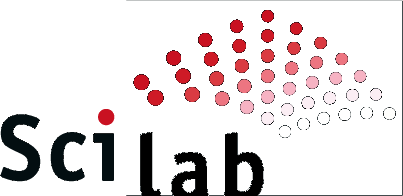
\includegraphics[height=.8cm]{png/logo_scilab}} 
\rotatebox{90}{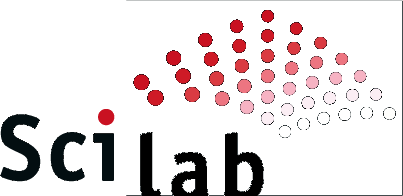
\includegraphics[height=.6cm]{png/logo_scilab}} 
        {\color{violetf}\vrule width 3pt}%
        \hspace{0pt}%must no space.
        \fboxsep=\FrameSep\colorbox{violetc}%
    }%
    \MakeFramed{\hsize #1 \advance\hsize-\width\FrameRestore}%
}%
{\endMakeFramed}%

\newenvironment{pseudo}[1][\hsize]%
{%
    \def\FrameCommand%
    {%
\rotatebox{90}{\textit{\textsf{Pseudo Code}}} 
        {\color{violetf}\vrule width 3pt}%
        \hspace{0pt}%must no space.
        \fboxsep=\FrameSep\colorbox{violetc}%
    }%
    \MakeFramed{\hsize #1 \advance\hsize-\width\FrameRestore}%
}%
{\endMakeFramed}%

\newenvironment{py}[1][\hsize]%
{%
    \def\FrameCommand%
    {%
%\rotatebox{90}{\textit{\textsf{Python}}} 
\rotatebox{90}{
\includegraphics[height=.6cm]{png/logo_python}} 
        {\color{violetf}\vrule width 3pt}%
        \hspace{0pt}%must no space.
        \fboxsep=\FrameSep\colorbox{violetc}%
    }%
    \MakeFramed{\hsize #1 \advance\hsize-\width\FrameRestore}%
}%
{\endMakeFramed}%


\newenvironment{corrige}[1][\hsize]%
{%
    \def\FrameCommand
    {%
\rotatebox{90}{\textit{\textsf{Correction}}} 
        {\color{violetf}\vrule width 3pt}%
        \hspace{0pt}%must no space.
        \fboxsep=\FrameSep\colorbox{violetc}%
    }%
    \MakeFramed{\hsize#1\advance\hsize-\width\FrameRestore}%
}%
{\endMakeFramed}%



\newenvironment{rem}[1][\hsize]%
{%
    \def\FrameCommand
    {%
\rotatebox{90}{\textit{\textsf{Remarque}}} 
        {\color{bleuf}\vrule width 3pt}%
        \hspace{0pt}%must no space.
        \fboxsep=\FrameSep\colorbox{bleuc}%
    }%
    \MakeFramed{\hsize#1\advance\hsize-\width\FrameRestore}%
}%
{\endMakeFramed}%


\newenvironment{savoir}[1][\hsize]%
{%
    \def\FrameCommand
    {%
\rotatebox{90}{\textit{\textsf{Savoir}}} 
        {\color{bleuf}\vrule width 3pt}%
        \hspace{0pt}%must no space.
        \fboxsep=\FrameSep\colorbox{bleuc}%
    }%
    \MakeFramed{\hsize#1\advance\hsize-\width\FrameRestore}%
}%
{\endMakeFramed}%

\newenvironment{prob}[1][\hsize]%
{%
    \def\FrameCommand%
    {%
\rotatebox{90}{\textit{\textsf{ Problématique}}} 
        {\color{rougef}\vrule width 3pt}%
        \hspace{0pt}%must no space.
        \fboxsep=\FrameSep\colorbox{rougec}%
    }%
    \MakeFramed{\hsize#1\advance\hsize-\width\FrameRestore}%
}%
{\endMakeFramed}%

\newenvironment{obj}[1][\hsize]%
{%
    \def\FrameCommand%
    {%
\rotatebox{90}{\textit{\textsf{Objectifs}}} 
        {\color{rougef}\vrule width 3pt}%
        \hspace{0pt}%must no space.
        \fboxsep=\FrameSep\colorbox{rougec}%
    }%
    \MakeFramed{\hsize#1\advance\hsize-\width\FrameRestore}%
}%
{\endMakeFramed}%

\newenvironment{defi}[1][\hsize]%
{%
    \def\FrameCommand%
    {%
\rotatebox{90}{\textit{\textsf{Définition\\}}} 
        {\color{bleuf}\vrule width 3pt}%
        \hspace{0pt}%must no space.
        \fboxsep=\FrameSep\colorbox{bleuc}%
    }%
    \MakeFramed{\hsize#1\advance\hsize-\width\FrameRestore}%
}%
{\endMakeFramed}%


\newenvironment{demo}[1][\hsize]%
{%
    \def\FrameCommand%
    {%
\rotatebox{90}{\textit{\textsf{Démonstration\\}}} 
        {\color{bleuf}\vrule width 3pt}%
        \hspace{0pt}%must no space.
        \fboxsep=\FrameSep\colorbox{bleuc}%
    }%
    \MakeFramed{\hsize#1\advance\hsize-\width\FrameRestore}%
}%
{\endMakeFramed}%


\newenvironment{hypo}[1][\hsize]%
{%
    \def\FrameCommand%
    {%
\rotatebox{90}{\textit{\textsf{Hypothèse\\}}} 
        {\color{bleuf}\vrule width 3pt}%
        \hspace{0pt}%must no space.
        \fboxsep=\FrameSep\colorbox{bleuc}%
    }%
    \MakeFramed{\hsize#1\advance\hsize-\width\FrameRestore}%
}%
{\endMakeFramed}%


\newenvironment{prop}[1][\hsize]%
{%
    \def\FrameCommand%
    {%
\rotatebox{90}{\textit{\textsf{Propriété\\}}} 
        {\color{bleuf}\vrule width 3pt}%
        \hspace{0pt}%must no space.
        \fboxsep=\FrameSep\colorbox{bleuc}%
    }%
    \MakeFramed{\hsize#1\advance\hsize-\width\FrameRestore}%
}%
{\endMakeFramed}%

\newenvironment{props}[1][\hsize]%
{%
    \def\FrameCommand%
    {%
\rotatebox{90}{\textit{\textsf{Propriétés\\}}} 
        {\color{bleuf}\vrule width 3pt}%
        \hspace{0pt}%must no space.
        \fboxsep=\FrameSep\colorbox{bleuc}%
    }%
    \MakeFramed{\hsize#1\advance\hsize-\width\FrameRestore}%
}%
{\endMakeFramed}%

\newenvironment{exemple}[1][\hsize]%
{%
    \def\FrameCommand%
    {%
\rotatebox{90}{\textit{\textsf{Exemple\\}}} 
        {\color{vertf}\vrule width 3pt}%
        \hspace{0pt}%must no space.
        \fboxsep=\FrameSep\colorbox{vertc}%
    }%
    \MakeFramed{\hsize#1\advance\hsize-\width\FrameRestore}%
}%
{\endMakeFramed}%

\newenvironment{resultat}[1][\hsize]%
{%
    \def\FrameCommand%
    {%
\rotatebox{90}{\textit{\textsf{Résultat\\}}} 
        {\color{rougef}\vrule width 3pt}%
        \hspace{0pt}%must no space.
        \fboxsep=\FrameSep\colorbox{rougec}%
    }%
    \MakeFramed{\hsize#1\advance\hsize-\width\FrameRestore}%
}%
{\endMakeFramed}%

\newenvironment{methode}[1][\hsize]%
{%
    \def\FrameCommand%
    {%
\rotatebox{90}{\textit{\textsf{Méthode\\}}} 
        {\color{rougef}\vrule width 3pt}%
        \hspace{0pt}%must no space.
        \fboxsep=\FrameSep\colorbox{rougec}%
    }%
    \MakeFramed{\hsize#1\advance\hsize-\width\FrameRestore}%
}%
{\endMakeFramed}%

\newenvironment{theo}[1][\hsize]%
{%
    \def\FrameCommand%
    {%
\rotatebox{90}{\textit{\textsf{Théorème\\}}} 
        {\color{rougef}\vrule width 3pt}%
        \hspace{0pt}%must no space.
        \fboxsep=\FrameSep\colorbox{rougec}%
    }%
    \MakeFramed{\hsize#1\advance\hsize-\width\FrameRestore}%
}%
{\endMakeFramed}%

\newenvironment{warn}[1][\hsize]%
{%
    \def\FrameCommand%
    {%
\rotatebox{90}{\textit{\textsf{Attention\\}}} 
        {\color{rougef}\vrule width 3pt}%
        \hspace{0pt}%must no space.
        \fboxsep=\FrameSep\colorbox{rougec}%
    }%
    \MakeFramed{\hsize#1\advance\hsize-\width\FrameRestore}%
}%
{\endMakeFramed}%

% \usepackage{pstricks}
%\usepackage{minitoc}
% \setcounter{minitocdepth}{4}

\setcounter{tocdepth}{2}

% \mtcselectlanguage{french} 

%\usepackage{draftcopy}% "Brouillon"
% \usepackage{floatflt}
\usepackage{psfrag}
%\usepackage{listings} % Permet d'insérer du code de programmation
\renewcommand{\baselinestretch}{1.2}

% Changer la numérotation des figures :
% ------------------------------------
% \makeatletter
% \renewcommand{\thefigure}{\ifnum \c@section>\z@ \thesection.\fi
%  \@arabic\c@figure}
% \@addtoreset{figure}{section}
% \makeatother
 


%%%%%%%%%%%%
% Définition des vecteurs %
%%%%%%%%%%%%
 \newcommand{\vect}[1]{\overrightarrow{#1}}

%%%%%%%%%%%%
% Définition des torseusr %
%%%%%%%%%%%%

 \newcommand{\torseur}[1]{%
\left\{{#1}\right\}
}

\newcommand{\torseurcin}[3]{%
\left\{\mathcal{#1} \left(#2/#3 \right) \right\}
}

\newcommand{\torseurstat}[3]{%
\left\{\mathcal{#1} \left(#2\rightarrow #3 \right) \right\}
}

 \newcommand{\torseurc}[8]{%
%\left\{#1 \right\}=
\left\{
{#1}
\right\}
 = 
\left\{%
\begin{array}{cc}%
{#2} & {#5}\\%
{#3} & {#6}\\%
{#4} & {#7}\\%
\end{array}%
\right\}_{#8}%
}

 \newcommand{\torseurcol}[7]{
\left\{%
\begin{array}{cc}%
{#1} & {#4}\\%
{#2} & {#5}\\%
{#3} & {#6}\\%
\end{array}%
\right\}_{#7}%
}

 \newcommand{\torseurl}[3]{%
%\left\{\mathcal{#1}\right\}_{#2}=%
\left\{%
\begin{array}{l}%
{#1} \\%
{#2} %
\end{array}%
\right\}_{#3}%
}

 \newcommand{\vectv}[3]{%
\vect{V\left( {#1} \in {#2}/{#3}\right)}
}


\newcommand{\vectf}[2]{%
\vect{R\left( {#1} \rightarrow {#2}\right)}
}

\newcommand{\vectm}[3]{%
\vect{\mathcal{M}\left( {#1}, {#2} \rightarrow {#3}\right)}
}


 \newcommand{\vectg}[3]{%
\vect{\Gamma \left( {#1} \in {#2}/{#3}\right)}
}

 \newcommand{\vecto}[2]{%
\vect{\Omega\left( {#1}/{#2}\right)}
}
% }$$\left\{\mathcal{#1} \right\}_{#2} =%
% \left\{%
% \begin{array}{c}%
%  #3 \\%
%  #4 %
% \end{array}%
% \right\}_{#5}}

%  ------------------------------------------
% | Modification du formatage des sections : | 
%  ------------------------------------------

% Grands titres :
% ---------------

\newcommand{\titre}[1]{%
\begin{center}
      \bigskip
      \rule{\textwidth}{1pt}
      \par\vspace{0.1cm}
      
      \textbf{\large #1}
      \par\rule{\textwidth}{1pt}
    \end{center}
    \bigskip
  }

% Supprime le numéro du chapitre dans la numérotation des sections:
% -----------------------------------------------------------------
\makeatletter
\renewcommand{\thesection}{\@arabic\c@section}
\makeatother


% \titleformat{\chapter}[display]
% {\normalfont\Large\filcenter}
% {}
% {1pc}
% {\titlerule[1pt]
%   \vspace{1pc}%
%   \Huge}[\vspace{1ex}%
% \titlerule]


%%%% Chapitres Comme PY Pechard %%%%%%%%%
% numéro du chapitre
\DeclareFixedFont{\chapnumfont}{OT1}{phv}{b}{n}{80pt}
% pour le mot « Chapitre »
\DeclareFixedFont{\chapchapfont}{OT1}{phv}{m}{it}{40pt}
% pour le titre
\DeclareFixedFont{\chaptitfont}{T1}{phv}{b}{n}{25pt}

\definecolor{gris}{gray}{0.75}
\titleformat{\chapter}[display]%
	{\sffamily}%
	{\filleft\chapchapfont\color{gris}\chaptertitlename\
	\\
	\vspace{12pt}
	\chapnumfont\thechapter}%
	{16pt}%
	{\filleft\chaptitfont}%
	[\vspace{6pt}\titlerule\titlerule\titlerule]

%%%%  Fin Chapitres Comme PY Pechard %%%%%%%%%


% Section, subsection, subsubsection sans serifs :
% % ----------------------------------------------

% \makeatletter
% \renewcommand{\section}{\@startsection{section}{0}{0mm}%
% {\baselineskip}{.3\baselineskip}%
% {\normalfont\sffamily\Large\textbf}}%
% \makeatother

\makeatletter
\renewcommand{\@seccntformat}[1]{{\textcolor{bleu}{\csname
the#1\endcsname}\hspace{0.5em}}}
\makeatother

\makeatletter
\renewcommand{\section}{\@startsection{section}{1}{\z@}%
                       {-4ex \@plus -1ex \@minus -.4ex}%
                       {1ex \@plus.2ex }%
                       {\normalfont\Large\sffamily\bfseries}}%
\makeatother
 
\makeatletter
\renewcommand{\subsection}{\@startsection {subsection}{2}{\z@}
                          {-3ex \@plus -0.1ex \@minus -.4ex}%
                          {0.5ex \@plus.2ex }%
                          {\normalfont\large\sffamily\bfseries}}
\makeatother
 
\makeatletter
\renewcommand{\subsubsection}{\@startsection {subsubsection}{3}{\z@}
                          {-2ex \@plus -0.1ex \@minus -.2ex}%
                          {0.2ex \@plus.2ex }%
                          {\normalfont\large\sffamily\bfseries}}
\makeatother
 
\makeatletter             
\renewcommand{\paragraph}{\@startsection{paragraph}{4}{\z@}%
                                    {-2ex \@plus-.2ex \@minus .2ex}%
                                    {0.1ex}%               
{\normalfont\sffamily\bfseries}}
\makeatother
 

\makeatletter             
\renewcommand{\subparagraph}{\@startsection{subparagraph}{5}{\z@}%
                                    {-2ex \@plus-.2ex \@minus .2ex}%
                                    {0.1ex}%               
{\normalfont\bfseries Question }}
\makeatother

\renewcommand{\thesubparagraph}{\arabic{subparagraph}} 
\makeatletter

\setcounter{secnumdepth}{5}
%\renewcommand{\subparagraph}{\@startsection{subparagraph}{5}{\z@}%
%                                       {-2ex \@plus-.1ex \@minus .2ex}%
%                                       {0.1ex}%
%				    {\normalfont\normalsize\sffamily\bfseries}}
%\makeatletter
% \makeatletter
% \renewcommand{\subsection}{\@startsection{subsection}{1}{2mm}%
% {\baselineskip}{.3\baselineskip}%
% {\normalfont\sffamily\large\textbf}}%
% \makeatother
% 
% \makeatletter
% \renewcommand{\subsubsection}{\@startsection{subsubsection}{2}{4mm}%
% {\baselineskip}{.15\baselineskip}%
% {\normalfont\sffamily\large\textbf}}%
% \makeatother
% 
% \makeatletter
% \renewcommand{\paragraph}{\@startsection{paragraph}{3}{6mm}%
% {\baselineskip}{.15\baselineskip}%
% {\normalfont\sffamily\large\textbf}}%
% \makeatother
 



%  --------
% | Marges |
%  --------


% \setmarginsrb{2.5cm}{1.5cm}{2.5cm}{2cm}{1cm}{1cm}{1cm}{1cm}
\setmarginsrb{1.5cm}{1cm}{1cm}{1.5cm}{1cm}{1cm}{1cm}{1cm}

% Changer les marges localement :
% -----------------------------
\newenvironment{changemargin}[2]{\begin{list}{}{%
\setlength{\topsep}{0pt}%
\setlength{\leftmargin}{0pt}%
\setlength{\rightmargin}{0pt}%
\setlength{\listparindent}{\parindent}%
\setlength{\itemindent}{\parindent}%
\setlength{\parsep}{0pt plus 1pt}%
\addtolength{\leftmargin}{#1}%
\addtolength{\rightmargin}{#2}%
}\item }{\end{list}}



\usepackage{pst-solides3d}
\usepackage{titletoc}
\titlecontents{chapter}[+3pc]
  {\addvspace{10pt}\sffamily\bfseries}
{\contentslabel[{\pscirclebox[fillstyle=solid,fillcolor=gray!25,
linecolor=gray!25,framesep=4pt]{\textcolor{white}{\thecontentslabel}}}]{2.5pc}}
  {}
  {\dotfill \normalfont\thecontentspage\ }

\titlecontents{section}[3pc]
  {\addvspace{2pt}\sffamily}
  {\contentslabel[\thecontentslabel]{1.8pc}}
  {}
  {\dotfill \normalfont\thecontentspage\ }

\titlecontents{subsection}[5pc]
  {\addvspace{2pt}\sffamily}
  {\contentslabel[\thecontentslabel]{1.8pc}}
  {}
  {\dotfill \normalfont\thecontentspage\ }

\titlecontents{subsubsection}[8pc]
  {\addvspace{2pt}\sffamily}
  {\contentslabel[\thecontentslabel]{3pc}}
  {}
  {\dotfill \normalfont\thecontentspage\ }
%{\;\titlerule\;\normalfont\thecontentspage\ }

\titlecontents{paragraph}[9pc]
  {\addvspace{2pt}\sffamily}
  {\contentslabel[\thecontentslabel]{3.5pc}}
  {}
  {\dotfill \normalfont\thecontentspage\ }



%\usepackage{algorithm}
%\usepackage{algorithmic}
\usepackage[french]{algorithm2e}

\SetKwBlock{Fonction}{Début Fonction}{Fin Fonction}
\SetKwComment{Comment}{start}{end}
% Python sources

\usepackage{listings}
\lstloadlanguages{R}   % pour regler les pb d accent utf8 dans les codes
\lstset{language=R} % pour regler les pb d accent utf8 dans les codes

\usepackage{textcomp}
\usepackage{setspace}
%\usepackage{palatino}

%\usepackage{color}
\definecolor{Bleu}{rgb}{0.1,0.1,1.0}
\definecolor{Noir}{rgb}{0,0,0}
\definecolor{Grau}{rgb}{0.5,0.5,0.5}
\definecolor{DunkelGrau}{rgb}{0.15,0.15,0.15}
\definecolor{Hellbraun}{rgb}{0.5,0.25,0.0}
\definecolor{Magenta}{rgb}{1.0,0.0,1.0}
\definecolor{Gris}{gray}{0.5}
\definecolor{Vert}{rgb}{0,0.5,0}
\definecolor{SourceHintergrund}{rgb}{1,1.0,0.95}


%
\renewcommand{\lstlistlistingname}{Listings}
\renewcommand{\lstlistingname}{Listing}

\lstnewenvironment{python}[1][]{
\lstset{
%escapeinside={\%*}{*)},
%inputencoding=utf8,   % pour regler les pb d accent utf8 dans les codes
%extendedchars=true,   % pour regler les pb d accent utf8 dans les codes
language=python,
basicstyle=\sffamily\footnotesize, 	
stringstyle=\color{red}, 
showstringspaces=false, 
alsoletter={1234567890},
otherkeywords={\ , \}, \{},
keywordstyle=\color{blue},
emph={access,and,break,class,continue,def,del,elif ,else,
except,exec,finally,for,from,global,if,import,in,i s,
lambda,not,or,pass,print,raise,return,try,while},
emphstyle=\color{black}\bfseries,
emph={[2]True, False, None, self},
emphstyle=[2]\color{olive},
emph={[3]from, import, as},
emphstyle=[3]\color{blue},
upquote=true,
columns=flexible, % pour empecher d'avoir un espacement mono
morecomment=[s]{"""}{"""},
commentstyle=\color{Hellbraun}\slshape, 
%emph={[4]1, 2, 3, 4, 5, 6, 7, 8, 9, 0},
emphstyle=[4]\color{blue},
literate=*{:}{{\textcolor{blue}:}}{1}
{=}{{\textcolor{blue}=}}{1}
{-}{{\textcolor{blue}-}}{1}
{+}{{\textcolor{blue}+}}{1}
{*}{{\textcolor{blue}*}}{1}
{!}{{\textcolor{blue}!}}{1}
{(}{{\textcolor{blue}(}}{1}
{)}{{\textcolor{blue})}}{1}
{[}{{\textcolor{blue}[}}{1}
{]}{{\textcolor{blue}]}}{1}
{<}{{\textcolor{blue}<}}{1}
{>}{{\textcolor{blue}>}}{1}
{COMPLETER}{{\textcolor{red}COMPLETER}}{1},
literate=%
            {é}{{\'{e}}}1
            {è}{{\`{e}}}1
            {ê}{{\^{e}}}1
            {ë}{{\¨{e}}}1
            {û}{{\^{u}}}1
            {ù}{{\`{u}}}1
            {â}{{\^{a}}}1
            {à}{{\`{a}}}1
            {î}{{\^{i}}}1
            {ç}{{\c{c}}}1
            {Ç}{{\c{C}}}1
            {É}{{\'{E}}}1
            {Ê}{{\^{E}}}1
            {À}{{\`{A}}}1
            {Â}{{\^{A}}}1
            {Î}{{\^{I}}}1, % pour regler les pb d accent utf8 dans les codes
%framexleftmargin=1mm, framextopmargin=1mm, frame=shadowbox, rulesepcolor=\color{blue},#1
%backgroundcolor=\color{SourceHintergrund}, 
%framexleftmargin=1mm, framexrightmargin=1mm, framextopmargin=1mm, frame=single, framerule=1pt, rulecolor=\color{black},#1
}}{}



\lstnewenvironment{scilab}[1][]{
\lstset{
language=scilab,
basicstyle=\sffamily\footnotesize, 	
stringstyle=\color{red}, 
showstringspaces=false, 
alsoletter={1234567890},
otherkeywords={\ , \}, \{},
keywordstyle=\color{blue},
emph={access,and,break,class,continue,def,del,elif ,else,
except,exec,finally,for,from,global,if,import,in,i s,
lambda,not,or,pass,print,raise,return,try,while,Debut},
emphstyle=\color{black}\bfseries,
emph={[2]True, False, None, self},
emphstyle=[2]\color{olive},
emph={[3]from, import, as},
emphstyle=[3]\color{blue},
upquote=true,
columns=flexible, % pour empecher d'avoir un espacement mono
morecomment=[s]{"""}{"""},
commentstyle=\color{Hellbraun}\slshape, 
%emph={[4]1, 2, 3, 4, 5, 6, 7, 8, 9, 0},
emphstyle=[4]\color{blue},
literate=*{:}{{\textcolor{blue}:}}{1}
{=}{{\textcolor{blue}=}}{1}
{-}{{\textcolor{blue}-}}{1}
{+}{{\textcolor{blue}+}}{1}
{*}{{\textcolor{blue}*}}{1}
{!}{{\textcolor{blue}!}}{1}
{(}{{\textcolor{blue}(}}{1}
{)}{{\textcolor{blue})}}{1}
{[}{{\textcolor{blue}[}}{1}
{]}{{\textcolor{blue}]}}{1}
{<}{{\textcolor{blue}<}}{1}
{>}{{\textcolor{blue}>}}{1},
%framexleftmargin=1mm, framextopmargin=1mm, frame=shadowbox, rulesepcolor=\color{blue},#1
%backgroundcolor=\color{SourceHintergrund}, 
%framexleftmargin=1mm, framexrightmargin=1mm, framextopmargin=1mm, frame=single, framerule=1pt, rulecolor=\color{black},#1
}}{}


\lstdefinestyle{stylepython}{%
escapeinside={\%*}{*)},
inputencoding=utf8,   % pour regler les pb d accent utf8 dans les codes
extendedchars=true,   % pour regler les pb d accent utf8 dans les codes
language=python,
basicstyle=\sffamily\footnotesize, 	
stringstyle=\color{red}, 
showstringspaces=false, 
alsoletter={1234567890},
otherkeywords={\ , \}, \{},
keywordstyle=\color{blue},
emph={access,and,break,class,continue,def,del,elif ,else,
except,exec,finally,for,from,global,if,import,in,i s,
lambda,not,or,pass,print,raise,return,try,while},
emphstyle=\color{black}\bfseries,
emph={[2]True, False, None, self},
emphstyle=[2]\color{green},
emph={[3]from, import, as},
emphstyle=[3]\color{blue},
upquote=true,
columns=flexible, % pour empecher d'avoir un espacement mono
morecomment=[s]{"""}{"""},
commentstyle=\color{Hellbraun}\slshape, 
%emph={[4]1, 2, 3, 4, 5, 6, 7, 8, 9, 0},
emphstyle=[4]\color{blue},
literate=*{:}{{\textcolor{blue}:}}{1}
{=}{{\textcolor{blue}=}}{1}
{-}{{\textcolor{blue}-}}{1}
{+}{{\textcolor{blue}+}}{1}
{*}{{\textcolor{blue}*}}{1}
{!}{{\textcolor{blue}!}}{1}
{(}{{\textcolor{blue}(}}{1}
{)}{{\textcolor{blue})}}{1}
{[}{{\textcolor{blue}[}}{1}
{]}{{\textcolor{blue}]}}{1}
{<}{{\textcolor{blue}<}}{1}
{>}{{\textcolor{blue}>}}{1}
{COMPLETER}{{\textcolor{red}COMPLETER}}{1},
literate=%
            {é}{{\'{e}}}1
            {è}{{\`{e}}}1
            {ê}{{\^{e}}}1
            {ë}{{\¨{e}}}1
            {û}{{\^{u}}}1
            {ù}{{\`{u}}}1
            {â}{{\^{a}}}1
            {à}{{\`{a}}}1
            {î}{{\^{i}}}1
            {ç}{{\c{c}}}1
            {Ç}{{\c{C}}}1
            {É}{{\'{E}}}1
            {Ê}{{\^{E}}}1
            {À}{{\`{A}}}1
            {Â}{{\^{A}}}1
            {Î}{{\^{I}}}1,
%numbers=left,                    % where to put the line-numbers; possible values are (none, left, right)
%numbersep=5pt,                   % how far the line-numbers are from the code
%numberstyle=\tiny\color{mygray}, % the style that is used for the line-numbers
}

%
%\renewcommand{\algorithmicrequire} {\textbf{\textsc{Entrées:}}}
%\renewcommand{\algorithmicensure}  {\textbf{\textsc{Sorties:}}}
%\renewcommand{\algorithmicwhile}   {\textbf{tantque}}
%\renewcommand{\algorithmicdo}      {\textbf{faire}}
%\renewcommand{\algorithmicendwhile}{\textbf{fin tantque}}
%\renewcommand{\algorithmicend}     {\textbf{fin}}
%\renewcommand{\algorithmicif}      {\textbf{si}}
%\renewcommand{\algorithmicendif}   {\textbf{finsi}}
%\renewcommand{\algorithmicelse}    {\textbf{sinon}}
%\renewcommand{\algorithmicthen}    {\textbf{alors}}
%\renewcommand{\algorithmicfor}     {\textbf{pour}}
%\renewcommand{\algorithmicforall}  {\textbf{pour tout}}
%\renewcommand{\algorithmicdo}      {\textbf{faire}}
%\renewcommand{\algorithmicendfor}  {\textbf{fin pour}}
%\renewcommand{\algorithmicloop}    {\textbf{boucler}}
%\renewcommand{\algorithmicendloop} {\textbf{fin boucle}}
%\renewcommand{\algorithmicrepeat}  {\textbf{répéter}}
%\renewcommand{\algorithmicuntil}   {\textbf{jusqu'à}}

\lstnewenvironment{termi}[1][]{
\lstset{
language=scilab,
basicstyle=\sffamily\footnotesize, 	
stringstyle=\color{red}, 
showstringspaces=false, 
alsoletter={1234567890},
otherkeywords={\ , \}, \{},
keywordstyle=\color{blue},
emph={access,and,break,class,continue,def,del,elif ,else,
except,exec,finally,for,from,global,if,import,in,i s,
lambda,not,or,pass,print,raise,return,try,while,Debut},
emphstyle=\color{black}\bfseries,
emph={[2]True, False, None, self},
emphstyle=[2]\color{green},
emph={[3]from, import, as},
emphstyle=[3]\color{blue},
upquote=true,
columns=flexible, % pour empecher d'avoir un espacement mono
morecomment=[s]{"""}{"""},
commentstyle=\color{Hellbraun}\slshape, 
%emph={[4]1, 2, 3, 4, 5, 6, 7, 8, 9, 0},
emphstyle=[4]\color{blue},
literate=*{:}{{\textcolor{blue}:}}{1}
{=}{{\textcolor{blue}=}}{1}
{-}{{\textcolor{blue}-}}{1}
{+}{{\textcolor{blue}+}}{1}
{*}{{\textcolor{blue}*}}{1}
{!}{{\textcolor{blue}!}}{1}
{(}{{\textcolor{blue}(}}{1}
{)}{{\textcolor{blue})}}{1}
{[}{{\textcolor{blue}[}}{1}
{]}{{\textcolor{blue}]}}{1}
{<}{{\textcolor{blue}<}}{1}
{>}{{\textcolor{blue}>}}{1},
%framexleftmargin=1mm, framextopmargin=1mm, frame=shadowbox, rulesepcolor=\color{blue},#1
%backgroundcolor=\color{SourceHintergrund}, 
%framexleftmargin=1mm, framexrightmargin=1mm, framextopmargin=1mm, frame=single, framerule=1pt, rulecolor=\color{black},#1
}}{}


%
%\renewcommand{\algorithmicrequire} {\textbf{\textsc{Entrées:}}}
%\renewcommand{\algorithmicensure}  {\textbf{\textsc{Sorties:}}}
%\renewcommand{\algorithmicwhile}   {\textbf{tantque}}
%\renewcommand{\algorithmicdo}      {\textbf{faire}}
%\renewcommand{\algorithmicendwhile}{\textbf{fin tantque}}
%\renewcommand{\algorithmicend}     {\textbf{fin}}
%\renewcommand{\algorithmicif}      {\textbf{si}}
%\renewcommand{\algorithmicendif}   {\textbf{finsi}}
%\renewcommand{\algorithmicelse}    {\textbf{sinon}}
%\renewcommand{\algorithmicthen}    {\textbf{alors}}
%\renewcommand{\algorithmicfor}     {\textbf{pour}}
%\renewcommand{\algorithmicforall}  {\textbf{pour tout}}
%\renewcommand{\algorithmicdo}      {\textbf{faire}}
%\renewcommand{\algorithmicendfor}  {\textbf{fin pour}}
%\renewcommand{\algorithmicloop}    {\textbf{boucler}}
%\renewcommand{\algorithmicendloop} {\textbf{fin boucle}}
%\renewcommand{\algorithmicrepeat}  {\textbf{répéter}}
%\renewcommand{\algorithmicuntil}   {\textbf{jusqu'à}}
%%%%%%%%%%%%
% Définition des vecteurs 
%%%%%%%%%%%%
\newcommand{\vect}[1]{\overrightarrow{#1}}
\newcommand{\axe}[2]{\left(#1,\vect{#2}\right)}
\newcommand{\rep}[5]{\mathcal{R}_{#1}=\left(#2,\vect{#3},\vect{#4},\vect{#5}\right)}
%%%%%%%%%%%%
% Définition des torseurs 
%%%%%%%%%%%%

\newcommand{\torseur}[1]{%
\left\{{#1}\right\}
}

\newcommand{\torseurcin}[3]{%
\left\{\mathcal{#1} \left(#2/#3 \right) \right\}
}

\newcommand{\torseurstat}[3]{%
\left\{\mathcal{#1} \left(#2\rightarrow #3 \right) \right\}
}

 \newcommand{\torseurc}[8]{%
%\left\{#1 \right\}=
\left\{
{#1}
\right\}
 = 
\left\{%
\begin{array}{cc}%
{#2} & {#5}\\%
{#3} & {#6}\\%
{#4} & {#7}\\%
\end{array}%
\right\}_{#8}%
}

 \newcommand{\torseurcol}[7]{
\left\{%
\begin{array}{cc}%
{#1} & {#4}\\%
{#2} & {#5}\\%
{#3} & {#6}\\%
\end{array}%
\right\}_{#7}%
}

 \newcommand{\torseurl}[3]{%
%\left\{\mathcal{#1}\right\}_{#2}=%
\left\{%
\begin{array}{l}%
{#1} \\%
{#2} %
\end{array}%
\right\}_{#3}%
}

 \newcommand{\vectv}[3]{%
\vect{V\left( {#1} \in {#2}/{#3}\right)}
}


\newcommand{\vectf}[2]{%
\vect{R\left( {#1} \rightarrow {#2}\right)}
}

\newcommand{\vectm}[3]{%
\vect{\mathcal{M}\left( {#1}, {#2} \rightarrow {#3}\right)}
}


 \newcommand{\vectg}[3]{%
\vect{\Gamma \left( {#1} \in {#2}/{#3}\right)}
}

 \newcommand{\vecto}[2]{%
\vect{\Omega\left( {#1}/{#2}\right)}
}
% }$$\left\{\mathcal{#1} \right\}_{#2} =%
% \left\{%
% \begin{array}{c}%
%  #3 \\%
%  #4 %
% \end{array}%
% \right\}_{#5}}
\setcounter{tocdepth}{2}
% \mtcselectlanguage{french} 


%  ------------------------------------------
% | Modification du formatage des sections : | 
%  ------------------------------------------

% Grands titres :
% ---------------

\newcommand{\titre}[1]{%
\begin{center}
      \bigskip
      \rule{\textwidth}{1pt}
      \par\vspace{0.1cm}
      
      \textbf{\large #1}
      \par\rule{\textwidth}{1pt}
    \end{center}
    \bigskip
  }

% Supprime le numéro du chapitre dans la numérotation des sections:
% -----------------------------------------------------------------
\makeatletter
\renewcommand{\thesection}{\@arabic\c@section}
\makeatother


% \titleformat{\chapter}[display]
% {\normalfont\Large\filcenter}
% {}
% {1pc}
% {\titlerule[1pt]
%   \vspace{1pc}%
%   \Huge}[\vspace{1ex}%
% \titlerule]


%%%% Chapitres Comme PY Pechard %%%%%%%%%
% numéro du chapitre
\DeclareFixedFont{\chapnumfont}{OT1}{phv}{b}{n}{80pt}
% pour le mot « Chapitre »
\DeclareFixedFont{\chapchapfont}{OT1}{phv}{m}{it}{40pt}
% pour le titre
\DeclareFixedFont{\chaptitfont}{T1}{phv}{b}{n}{25pt}

\definecolor{gris}{gray}{0.75}
\titleformat{\chapter}[display]%
	{\sffamily}%
	{\filleft\chapchapfont\color{gris}\chaptertitlename\
	\\
	\vspace{12pt}
	\chapnumfont\thechapter}%
	{16pt}%
	{\filleft\chaptitfont}%
	[\vspace{6pt}\titlerule\titlerule\titlerule]

%%%%  Fin Chapitres Comme PY Pechard %%%%%%%%%


% Section, subsection, subsubsection sans serifs :
% % ----------------------------------------------

% \makeatletter
% \renewcommand{\section}{\@startsection{section}{0}{0mm}%
% {\baselineskip}{.3\baselineskip}%
% {\normalfont\sffamily\Large\textbf}}%
% \makeatother

\makeatletter
\renewcommand{\@seccntformat}[1]{{\textcolor{bleu}{\csname
the#1\endcsname}\hspace{0.5em}}}
\makeatother

\makeatletter
\renewcommand{\section}{\@startsection{section}{1}{\z@}%
                       {-4ex \@plus -1ex \@minus -.4ex}%
                       {1ex \@plus.2ex }%
                       {\normalfont\Large\sffamily\bfseries}}%
\makeatother
 
\makeatletter
\renewcommand{\subsection}{\@startsection {subsection}{2}{\z@}
                          {-3ex \@plus -0.1ex \@minus -.4ex}%
                          {0.5ex \@plus.2ex }%
                          {\normalfont\large\sffamily\bfseries}}
\makeatother
 
\makeatletter
\renewcommand{\subsubsection}{\@startsection {subsubsection}{3}{\z@}
                          {-2ex \@plus -0.1ex \@minus -.2ex}%
                          {0.2ex \@plus.2ex }%
                          {\normalfont\large\sffamily\bfseries}}
\makeatother
 
\makeatletter             
\renewcommand{\paragraph}{\@startsection{paragraph}{4}{\z@}%
                                    {-2ex \@plus-.2ex \@minus .2ex}%
                                    {0.1ex}%               
{\normalfont\sffamily\bfseries}}
\makeatother
 
 
\makeatletter             
\renewcommand{\subparagraph}{\@startsection{subparagraph}{5}{\z@}%
                                    {-2ex \@plus-.2ex \@minus .2ex}%
                                    {0.1ex}%               
{\normalfont\bfseries Question }}
\makeatother
\renewcommand{\thesubparagraph}{\arabic{subparagraph}} 
\makeatletter

\setcounter{secnumdepth}{5}





% Formatage de la table des matières 
% Paquets nécessaires : titletoc ?

% Chapitre spéciaux écrits dans un nombre cerclé dans la table des matières.
\titlecontents{chapter}[+3pc]
  {\addvspace{10pt}\sffamily\bfseries}
{\contentslabel[{\pscirclebox[fillstyle=solid,fillcolor=gray!25,
linecolor=gray!25,framesep=4pt]{\textcolor{white}{\thecontentslabel}}}]{2.5pc}}
  {}
  {\dotfill \normalfont\thecontentspage\ }

\titlecontents{section}[3pc]
  {\addvspace{2pt}\sffamily}
  {\contentslabel[\thecontentslabel]{1.8pc}}
  {}
  {\dotfill \normalfont\thecontentspage\ }

\titlecontents{subsection}[5pc]
  {\addvspace{2pt}\sffamily}
  {\contentslabel[\thecontentslabel]{1.8pc}}
  {}
  {\dotfill \normalfont\thecontentspage\ }

\titlecontents{subsubsection}[8pc]
  {\addvspace{2pt}\sffamily}
  {\contentslabel[\thecontentslabel]{3pc}}
  {}
  {\dotfill \normalfont\thecontentspage\ }
%{\;\titlerule\;\normalfont\thecontentspage\ }

\titlecontents{paragraph}[9pc]
  {\addvspace{2pt}\sffamily}
  {\contentslabel[\thecontentslabel]{3.5pc}}
  {}
  {\dotfill \normalfont\thecontentspage\ }

%pour avoir l indentation dans minipage
\newdimen\oldparindent\oldparindent=\parindent

\makeatletter
\def\@iiiminipage#1#2[#3]#4{%
  \noindent
  \leavevmode
  \@pboxswfalse
  \setlength\@tempdima{#4}%
  \def\@mpargs{{#1}{#2}[#3]{#4}}%
  \setbox\@tempboxa\vbox\bgroup
    \color@begingroup
      \hsize\@tempdima
      \textwidth\hsize \columnwidth\hsize
      \@parboxrestore
      \parindent=\oldparindent
      \def\@mpfn{mpfootnote}\def\thempfn{\thempfootnote}\c@mpfootnote\z@
      \let\@footnotetext\@mpfootnotetext
      \let\@listdepth\@mplistdepth \@mplistdepth\z@
      \@minipagerestore
      \@setminipage}
\makeatother

% Paquets requis : 

\definecolor{gris25}{gray}{0.75}
\definecolor{bleu}{RGB}{18,33,98}
\definecolor{bleuf}{RGB}{42,94,171}
\definecolor{bleuc}{RGB}{231,239,247}
\definecolor{rougef}{RGB}{185,18,27}
\definecolor{rougec}{RGB}{255,230,231}
\definecolor{vertf}{RGB}{103,126,82}
\definecolor{vertc}{RGB}{220,255,191}
\definecolor{violetf}{RGB}{112,48,160}
\definecolor{violetc}{RGB}{230,224,236}
\definecolor{jaunec}{RGB}{220,255,191}



\newenvironment{corrige}[1][\hsize]%
{%
    \def\FrameCommand%
    {%
\rotatebox{90}{\textit{\textsf{Corrigé}}} 
        {\color{violetf}\vrule width 3pt}%
        \hspace{0pt}%must no space.
        \fboxsep=\FrameSep\colorbox{violetc}%
    }%
    \MakeFramed{\hsize #1 \advance\hsize-\width\FrameRestore}%
}%
{\endMakeFramed}%

\newenvironment{sci}[1][\hsize]%
{%
    \def\FrameCommand%
    {%
%\rotatebox{90}{\textit{\textsf{Scilab}}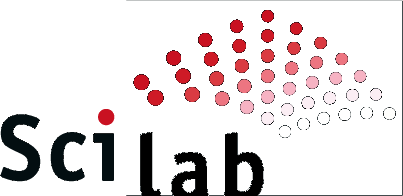
\includegraphics[height=.8cm]{png/logo_scilab}} 
\rotatebox{90}{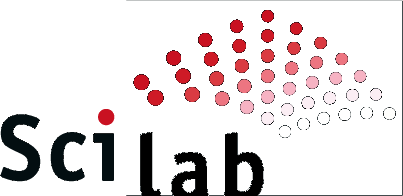
\includegraphics[height=.6cm]{png/logo_scilab}} 
        {\color{violetf}\vrule width 3pt}%
        \hspace{0pt}%must no space.
        \fboxsep=\FrameSep\colorbox{violetc}%
    }%
    \MakeFramed{\hsize #1 \advance\hsize-\width\FrameRestore}%
}%
{\endMakeFramed}%

\newenvironment{pseudo}[1][\hsize]%
{%
    \def\FrameCommand%
    {%
\rotatebox{90}{\textit{\textsf{Pseudo Code}}} 
        {\color{violetf}\vrule width 3pt}%
        \hspace{0pt}%must no space.
        \fboxsep=\FrameSep\colorbox{violetc}%
    }%
    \MakeFramed{\hsize #1 \advance\hsize-\width\FrameRestore}%
}%
{\endMakeFramed}%

\newenvironment{py}[1][\hsize]%
{%
    \def\FrameCommand%
    {%
%\rotatebox{90}{\textit{\textsf{Python}}} 
\rotatebox{90}{
\includegraphics[height=.6cm]{png/logo_python}} 
        {\color{violetf}\vrule width 3pt}%
        \hspace{0pt}%must no space.
        \fboxsep=\FrameSep\colorbox{violetc}%
    }%
    \MakeFramed{\hsize #1 \advance\hsize-\width\FrameRestore}%
}%
{\endMakeFramed}%


\newenvironment{term}[1][\hsize]%
{%
    \def\FrameCommand%
    {%
\rotatebox{90}{\textit{\textsf{Terminal}}} 
        {\color{violetf}\vrule width 3pt}%
        \hspace{0pt}%must no space.
        \fboxsep=\FrameSep\colorbox{violetc}%
    }%
    \MakeFramed{\hsize #1 \advance\hsize-\width\FrameRestore}%
}%
{\endMakeFramed}%


\newenvironment{rem}[1][\hsize]%
{%
    \def\FrameCommand
    {%
\rotatebox{90}{\textit{\textsf{Remarque}}} 
        {\color{bleuf}\vrule width 3pt}%
        \hspace{0pt}%must no space.
        \fboxsep=\FrameSep\colorbox{bleuc}%
    }%
    \MakeFramed{\hsize#1\advance\hsize-\width\FrameRestore}%
}%
{\endMakeFramed}%


\newenvironment{savoir}[1][\hsize]%
{%
    \def\FrameCommand
    {%
\rotatebox{90}{\textit{\textsf{Savoir}}} 
        {\color{bleuf}\vrule width 3pt}%
        \hspace{0pt}%must no space.
        \fboxsep=\FrameSep\colorbox{bleuc}%
    }%
    \MakeFramed{\hsize#1\advance\hsize-\width\FrameRestore}%
}%
{\endMakeFramed}%

\newenvironment{Objectif}[1][\hsize]%
{%
    \def\FrameCommand
    {%
\rotatebox{90}{\textit{\textsf{Objectif}}} 
        {\color{bleuf}\vrule width 3pt}%
        \hspace{0pt}%must no space.
        \fboxsep=\FrameSep\colorbox{bleuc}%
    }%
    \MakeFramed{\hsize#1\advance\hsize-\width\FrameRestore}%
}%
{\endMakeFramed}%

\newenvironment{prob}[1][\hsize]%
{%
    \def\FrameCommand%
    {%
\rotatebox{90}{\textit{\textsf{ Problématique}}} 
        {\color{rougef}\vrule width 3pt}%
        \hspace{0pt}%must no space.
        \fboxsep=\FrameSep\colorbox{rougec}%
    }%
    \MakeFramed{\hsize#1\advance\hsize-\width\FrameRestore}%
}%
{\endMakeFramed}%

\newenvironment{obj}[1][\hsize]%
{%
    \def\FrameCommand%
    {%
\rotatebox{90}{\textit{\textsf{Objectif}}} 
        {\color{rougef}\vrule width 3pt}%
        \hspace{0pt}%must no space.
        \fboxsep=\FrameSep\colorbox{rougec}%
    }%
    \MakeFramed{\hsize#1\advance\hsize-\width\FrameRestore}%
}%
{\endMakeFramed}%

\newenvironment{defi}[1][\hsize]%
{%
    \def\FrameCommand%
    {%
\rotatebox{90}{\textit{\textsf{Définition\\}}} 
        {\color{bleuf}\vrule width 3pt}%
        \hspace{0pt}%must no space.
        \fboxsep=\FrameSep\colorbox{bleuc}%
    }%
    \MakeFramed{\hsize#1\advance\hsize-\width\FrameRestore}%
}%
{\endMakeFramed}%


\newenvironment{demo}[1][\hsize]%
{%
    \def\FrameCommand%
    {%
\rotatebox{90}{\textit{\textsf{Démonstration\\}}} 
        {\color{bleuf}\vrule width 3pt}%
        \hspace{0pt}%must no space.
        \fboxsep=\FrameSep\colorbox{bleuc}%
    }%
    \MakeFramed{\hsize#1\advance\hsize-\width\FrameRestore}%
}%
{\endMakeFramed}%


\newenvironment{hypo}[1][\hsize]%
{%
    \def\FrameCommand%
    {%
\rotatebox{90}{\textit{\textsf{Hypothèse\\}}} 
        {\color{bleuf}\vrule width 3pt}%
        \hspace{0pt}%must no space.
        \fboxsep=\FrameSep\colorbox{bleuc}%
    }%
    \MakeFramed{\hsize#1\advance\hsize-\width\FrameRestore}%
}%
{\endMakeFramed}%


\newenvironment{prop}[1][\hsize]%
{%
    \def\FrameCommand%
    {%
\rotatebox{90}{\textit{\textsf{Propriété\\}}} 
        {\color{bleuf}\vrule width 3pt}%
        \hspace{0pt}%must no space.
        \fboxsep=\FrameSep\colorbox{bleuc}%
    }%
    \MakeFramed{\hsize#1\advance\hsize-\width\FrameRestore}%
}%
{\endMakeFramed}%

\newenvironment{props}[1][\hsize]%
{%
    \def\FrameCommand%
    {%
\rotatebox{90}{\textit{\textsf{Propriétés\\}}} 
        {\color{bleuf}\vrule width 3pt}%
        \hspace{0pt}%must no space.
        \fboxsep=\FrameSep\colorbox{bleuc}%
    }%
    \MakeFramed{\hsize#1\advance\hsize-\width\FrameRestore}%
}%
{\endMakeFramed}%

\newenvironment{exemple}[1][\hsize]%
{%
    \def\FrameCommand%
    {%
\rotatebox{90}{\textit{\textsf{Exemple\\}}} 
        {\color{vertf}\vrule width 3pt}%
        \hspace{0pt}%must no space.
        \fboxsep=\FrameSep\colorbox{vertc}%
    }%
    \MakeFramed{\hsize#1\advance\hsize-\width\FrameRestore}%
}%
{\endMakeFramed}%

\newenvironment{exercice}[1][\hsize]%
{%
    \def\FrameCommand%
    {%
\rotatebox{90}{\textit{\textsf{Exercice\\}}} 
        {\color{vertf}\vrule width 3pt}%
        \hspace{0pt}%must no space.
        \fboxsep=\FrameSep\colorbox{vertc}%
    }%
    \MakeFramed{\hsize#1\advance\hsize-\width\FrameRestore}%
}%
{\endMakeFramed}%

\newenvironment{Support}[1][\hsize]%
{%
    \def\FrameCommand%
    {%
\rotatebox{90}{\textit{\textsf{Support de cours\\}}} 
        {\color{vertf}\vrule width 3pt}%
        \hspace{0pt}%must no space.
        \fboxsep=\FrameSep\colorbox{jaunec}%
    }%
    \MakeFramed{\hsize#1\advance\hsize-\width\FrameRestore}%
}%
{\endMakeFramed}%

\newenvironment{resultat}[1][\hsize]%
{%
    \def\FrameCommand%
    {%
\rotatebox{90}{\textit{\textsf{Résultat\\}}} 
        {\color{rougef}\vrule width 3pt}%
        \hspace{0pt}%must no space.
        \fboxsep=\FrameSep\colorbox{rougec}%
    }%
    \MakeFramed{\hsize#1\advance\hsize-\width\FrameRestore}%
}%
{\endMakeFramed}%

\newenvironment{methode}[1][\hsize]%
{%
    \def\FrameCommand%
    {%
\rotatebox{90}{\textit{\textsf{Méthode\\}}} 
        {\color{rougef}\vrule width 3pt}%
        \hspace{0pt}%must no space.
        \fboxsep=\FrameSep\colorbox{rougec}%
    }%
    \MakeFramed{\hsize#1\advance\hsize-\width\FrameRestore}%
}%
{\endMakeFramed}%

\newenvironment{theo}[1][\hsize]%
{%
    \def\FrameCommand%
    {%
\rotatebox{90}{\textit{\textsf{Théorème\\}}} 
        {\color{rougef}\vrule width 3pt}%
        \hspace{0pt}%must no space.
        \fboxsep=\FrameSep\colorbox{rougec}%
    }%
    \MakeFramed{\hsize#1\advance\hsize-\width\FrameRestore}%
}%
{\endMakeFramed}%

\newenvironment{warn}[1][\hsize]%
{%
    \def\FrameCommand%
    {%
\rotatebox{90}{\textit{\textsf{Attention\\}}} 
        {\color{rougef}\vrule width 3pt}%
        \hspace{0pt}%must no space.
        \fboxsep=\FrameSep\colorbox{rougec}%
    }%
    \MakeFramed{\hsize#1\advance\hsize-\width\FrameRestore}%
}%
{\endMakeFramed}%

%Si le boolen xp est vrai : compilation pour xabi
%Sinon compilation Damien
\newboolean{xp}
\setboolean{xp}{true}

\newboolean{prof}
\setboolean{prof}{false}

\usepackage[%
    pdftitle={DM 8},
    pdfauthor={Xavier Pessoles},
    colorlinks=true,
    linkcolor=blue,
    citecolor=magenta]{hyperref}


\def\discipline{Sciences Industrielles de l'Ingénieur}
\def\xxtitre{\ifthenelse{\boolean{xp}}{
Devoir Maison 8
}{
Chapitre  -- }}

\def\xxsoustitre{\ifthenelse{\boolean{xp}}{
Mélangeur interne à rotors engrenants
}{
Partie  -- }}

\def\xxauteur{\ifthenelse{\boolean{xp}}{
Xavier \textsc{Pessoles} }{}}

\def\xxpied{\ifthenelse{\boolean{xp}}{
DM 8 -- \ifthenelse{\boolean{prof}}{Corrigé}{Sujet}}{
\xxtitre}}

\def\xxcathegorie{\ifthenelse{\boolean{xp}}{
2013 -- 2014 \\
Xavier \textsc{Pessoles}}{
Informatique - Cours}}





%---------------------------------------------------------------------------


\begin{document}

\ifthenelse{\boolean{xp}}{
\sloppy
\hyphenpenalty 10000


%------------- En tetes et Pieds de Pages ------------

\pagestyle{fancy}
\renewcommand{\headrulewidth}{0pt}
\fancyhead{}
\fancyhead[L]{%
\noindent\begin{minipage}[c]{2.6cm}%

\includegraphics[width=2cm]{png/logo_ptsi.png}%
\end{minipage}}


\fancyhead[C]{\rule{12cm}{.5pt}}


\fancyhead[R]{%
\noindent\begin{minipage}[c]{3cm}
\begin{flushright}
\footnotesize{\textit{\textsf{\discipline}}}%
\end{flushright}
\end{minipage}
}



\fancyhead[C]{\rule{12cm}{.5pt}}

\renewcommand{\footrulewidth}{0.2pt}

\fancyfoot[C]{\footnotesize{\bfseries \thepage}}
\fancyfoot[L]{%
\begin{minipage}[c]{.2\linewidth}
\noindent\footnotesize{{\xxauteur}}
\end{minipage}
}

\ifthenelse{\boolean{prof}}{%
\fancyfoot[R]{\footnotesize{\xxpied}}}

\begin{center}
 \huge\textsc{\xxtitre}
\end{center}

\begin{center}
 \LARGE\textsc{\xxsoustitre}
\end{center}

\vspace{.5cm}
}{\ifthenelse{\boolean{xp}}{
\usepackage[%
    pdftitle={OS et Environnement de développement},
    pdfauthor={Xavier Pessoles},
    colorlinks=true,
    linkcolor=blue,
    citecolor=magenta]{hyperref}}{
\usepackage[%
    pdftitle={OS et Environnement de développement},
    pdfauthor={Damien Iceta},
    colorlinks=true,
    linkcolor=blue,
    citecolor=magenta]{hyperref}}

\usepackage{pifont}
\usepackage{lastpage}

\newcommand{\axe}[2]{\left(#1,\vect{#2}\right)}
\newcommand{\rep}[5]{\mathcal{R}_{#1}=\left(#2,\vect{#3},\vect{#4},\vect{#5}\right)}

% \makeatletter \let\ps@plain\ps@empty \makeatother
%% DEBUT DU DOCUMENT
%% =================
\sloppy
\hyphenpenalty 10000

\newcommand{\Pointilles}[1][3]{%
\multido{}{#1}{\makebox[\linewidth]{\dotfill}\\[\parskip]
}}


\colorlet{shadecolor}{orange!15}

\newtheorem{theorem}{Theorem}


\begin{document}


\newboolean{prof}
\setboolean{prof}{true}
%------------- En tetes et Pieds de Pages ------------


\pagestyle{fancy}
%\renewcommand{\headrulewidth}{0}
\renewcommand{\headrulewidth}{0.2pt} %pour mettre le trait en haut

\fancyhead{}
\fancyhead[L]{
\footnotesize{{{\xxtitre}}}%
%\noindent\noindent\begin{minipage}[c]{2.6cm}
%\includegraphics[width=2.5cm]{png/logo.png}%
%\end{minipage}
}

%\fancyhead[C]{\rule{12cm}{.5pt}}  %pour mettre le petit trait en haut


\fancyhead[R]{%
\noindent\begin{minipage}[c]{3cm}
\begin{flushright}
\footnotesize{{{\xxcathegorie}}}%
\end{flushright}
\end{minipage}
}

\renewcommand{\footrulewidth}{0.2pt}

\fancyfoot[C]{\footnotesize{}}
\fancyfoot[L]{%
\begin{minipage}[l]{.2\linewidth}
\noindent\footnotesize{{\xxauteur}}
\end{minipage}
\begin{minipage}[c]{.15\linewidth}
%
\includegraphics[width=2cm]{png/logoCC.png}
\end{minipage}}

\ifthenelse{\boolean{prof}}{%
\fancyfoot[R]{\footnotesize{Page \thepage\   sur  \pageref{LastPage}}}}

\begin{center}
 \huge\textsc{\xxtitre}
\end{center}

\begin{center}
 \LARGE\textsc{\xxsoustitre}
\end{center}

\vspace{.5cm}}

\ifthenelse{\boolean{prof}}{\begin{center}
\textit{Éléments de corrigé -- Adapté du concours E3A -- PSI -- 2013}
\end{center}}{}

%\setlength{\parskip}{0ex plus 0.2ex minus 0ex}
% \renewcommand{\contentsname}{}
% \renewcommand{\baselinestretch}{1}
%
%\tableofcontents

 \renewcommand{\baselinestretch}{1.2}
\setlength{\parskip}{2ex plus 0.5ex minus 0.2ex}



\ifthenelse{\boolean{prof}}{}{
\begin{minipage}[c]{.45\linewidth}
\begin{center}
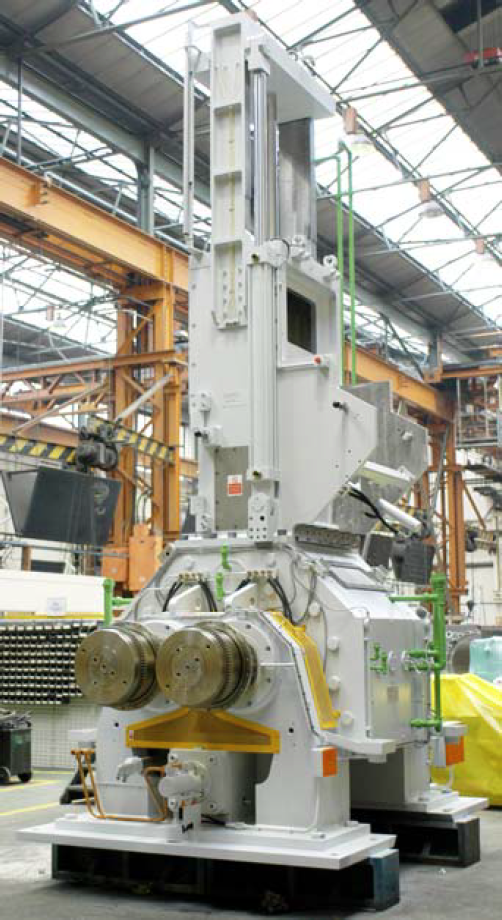
\includegraphics[width=.5\textwidth]{images/intermix}
\end{center}
\end{minipage} \hfill
\begin{minipage}[c]{.45\linewidth}
\begin{center}
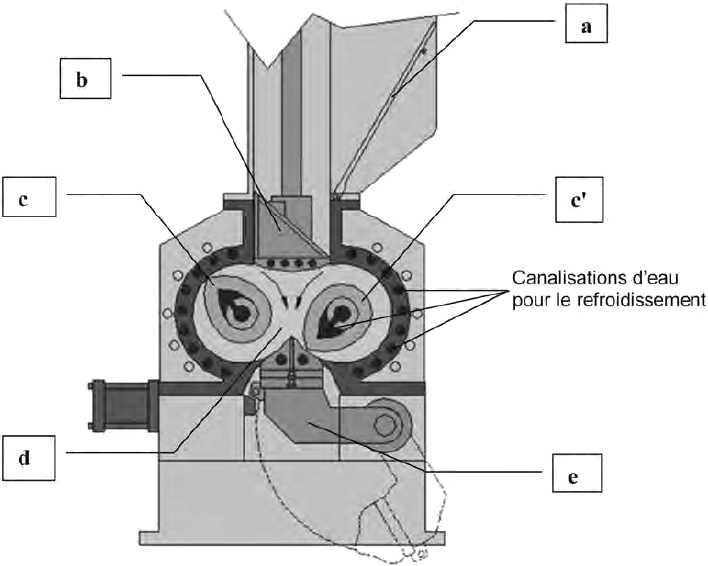
\includegraphics[width=\textwidth]{images/schema}
\end{center}
\end{minipage} 
}

\section{Présentation du mélangeur à rotors engrenants}
\ifthenelse{\boolean{prof}}{}{
Un mélangeur interne à rotors engrenants est une machine utilisée dans l'industrie pour effectuer le mélange du caoutchouc et d'additifs divers. Il est, par exemple, utilisé dans la fabrication des pneumatiques.
Nous nous intéresserons dans cette étude au modèle K5 de la société Farrel.

Le mélangeur est principalement constitué de :
\begin{itemize}
\item une porte de chargement du caoutchouc et des différents additifs (a);
\item un fouloir permettant de pousser les différents ingrédients vers la chambre de mélangeage (b);
\item deux rotors à axes parallèles tournant en sens inverses (c) et (c');
\item une chambre de mélangeage (d);
\item une porte de déchargement (e).
\end{itemize}

Le modèle K5 permet de mélanger 100 kg de matière dans une chambre ayant une contenance de 143 litres. Le mélangeur a une masse totale de 16 tonnes. La masse du moteur électrique entraînant les rotors est de 2,5 tonnes.

Les caractéristiques du mélange obtenu dépendent, en plus des caractéristiques des différents constituants, des conditions dans lesquelles s'effectue le mélange. Il est donc important de maîtriser, au cours des différentes phases du mélange, la vitesse de rotation des rotors et l'effort exercé par le fouloir tout en surveillant la température dans la chambre qui ne doit pas dépasser une valeur limite (pour que le mélange ne vulcanise pas dans le mélangeur).

\begin{center}
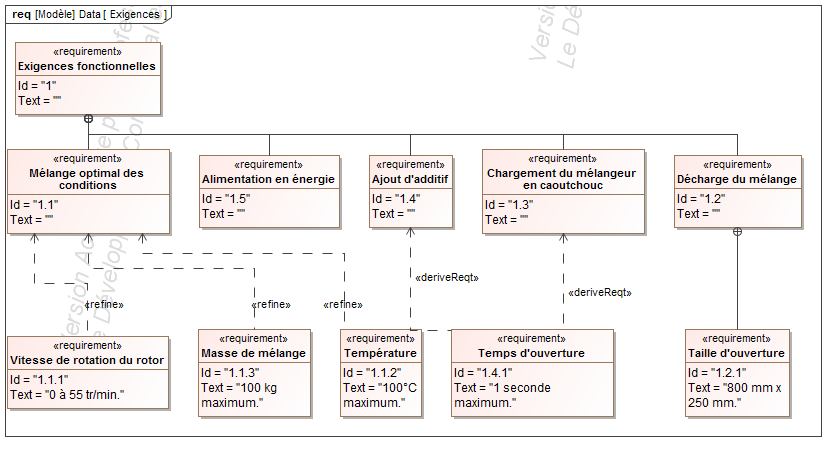
\includegraphics[width=.8\textwidth]{images/Exigences}
\end{center}
}

\section{Étude de la chaîne fonctionnelle de mise en mouvement des rotors}
\ifthenelse{\boolean{prof}}{}{
\begin{obj}
Vérifier le dimensionnement de l'actionneur. Choisir et régler un correcteur pour optimiser les performances de l'asservissement de vitesse participant à l'exigence 1.1.
\end{obj}}


\subsection{Construction du schéma bloc}
\ifthenelse{\boolean{prof}}{}{
\begin{obj}
Mettre en place la structure globale de l'asservissement de vitesse.
\end{obj}

L'asservissement en vitesse des rotors est représenté par le schéma suivant :

\begin{center}
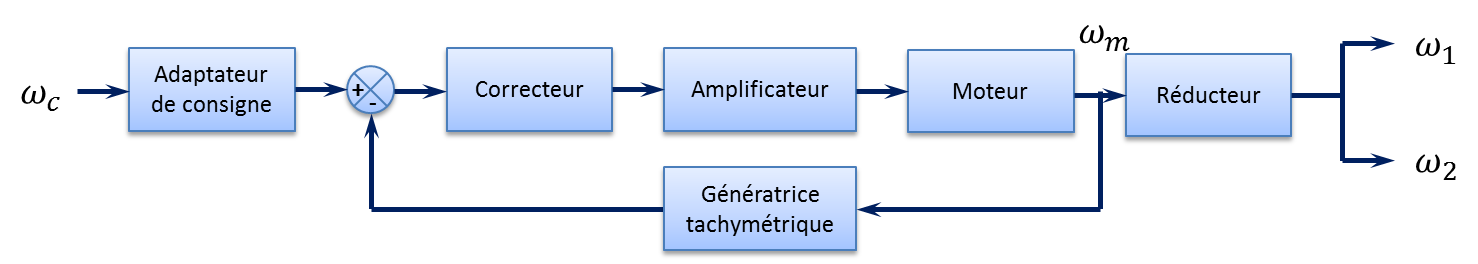
\includegraphics[width=.8\textwidth]{images/SchemaBloc}
\end{center}

$\omega_c$ : consigne de vitesse; $\omega_m$ : vitesse moteur ; $\omega_1$ : vitesse rotor 1 ; $\omega_2$ : vitesse rotor 2

\begin{rem}
Ces quatre vitesses sont des vitesses angulaires par rapport au bâti.
\end{rem}

On donne les équations suivantes caractérisant le moteur :
$$
C_m(t)+C_r(t) = J \dfrac{d\omega_m(t)}{dt}
\quad
u(t)=Ri(t)+L\dfrac{di(t)}{dt}+e(t)
\quad
C_m(t)=k_i i(t)
\quad 
e(t)=k_e\omega_m(t)
$$
\begin{itemize}
\item $R$ : résistance de l'induit;
\item $L$ : inductance de l'induit;
\item $u(t)$ : tension d'alimentation du moteur;
\item $i(t)$ : courant moteur;
\item $e(t)$ : force contre électromotrice;
\item $C_m(t)$ : couple disponible sur l'arbre moteur;
\item $C_r(t)$ : couple résistant ramené sur l'arbre moteur;
\item $\omega_m(t)$ : vitesse de rotation de l'arbre moteur;
\item $J$ : moment d'inertie ramené sur l'arbre moteur;
\item $k_e$ : constante de force contre électromotrice;
\item $k_i$ : constante de couple.
\end{itemize}

On notera $C_m(p)$, $C_r(p)$, $\Omega_m(p)$, $U(p)$, $I(p)$ et $E(p)$ les transformées de Laplace des différentes grandeurs physiques définies ci-dessus.}

% Question II.A.1
\subparagraph{}
\textit{En considérant que toutes les conditions initiales sont nulles, donner les quatre équations précédentes dans le domaine de Laplace.}
\ifthenelse{\boolean{prof}}{
\begin{corrige}
$$
C_m(p)+C_r(p) = J p\Omega_m(p)
\quad
U(p)=RI(p)+LpI(p)+E(p)
\quad
C_m(p)=k_i I(p)
\quad 
E(p)=k_e\Omega_m(p)
$$

\end{corrige}}{}

% Question II.A.2
\subparagraph{}
\textit{Remplir les fonctions de transfert des cases $d$, $e$, $f$ et $g$ ainsi que les trois grandeurs physiques manquantes (zones grisées) sur le schéma-bloc fourni sur le cahier réponses.}
\ifthenelse{\boolean{prof}}{
\begin{corrige}
\begin{center}
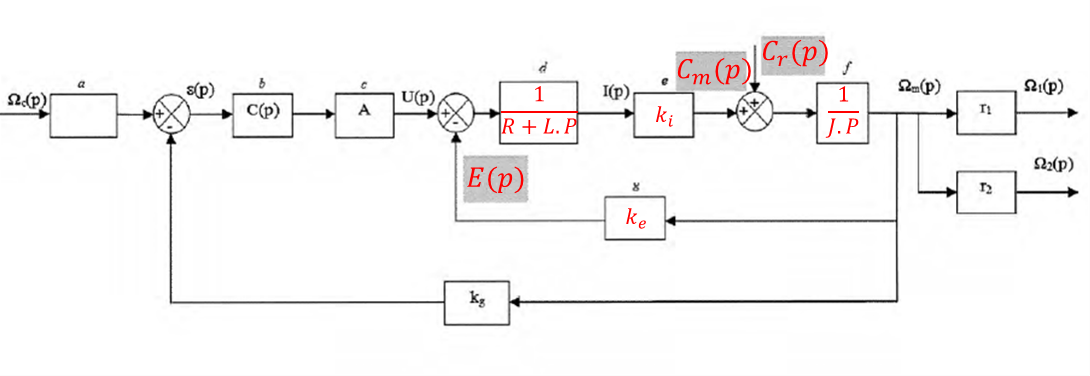
\includegraphics[width=.8\textwidth]{images/cor_blocs}
\end{center}
\end{corrige}}{}
\ifthenelse{\boolean{prof}}{}{
\begin{center}
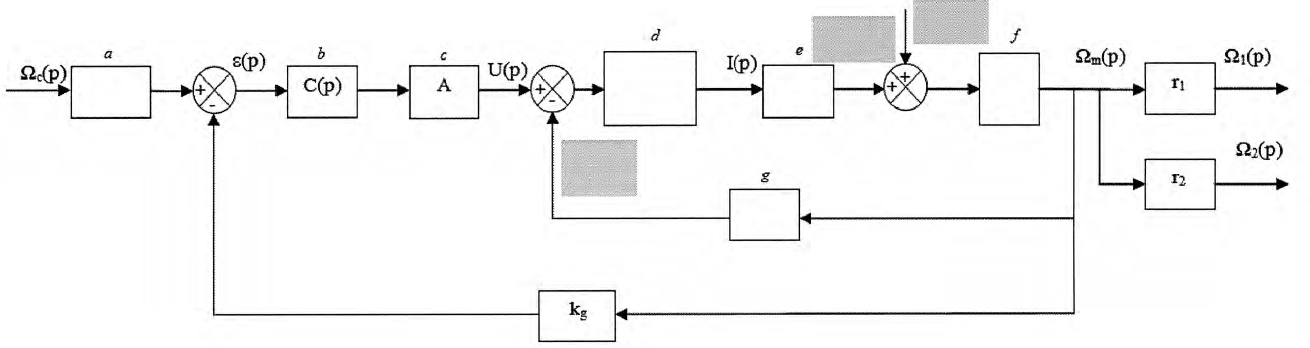
\includegraphics[width=.8\textwidth]{images/qiia2}
\end{center}


Le schéma cinématique et les caractéristiques du réducteur sont fournis ci-dessous.

\begin{center}
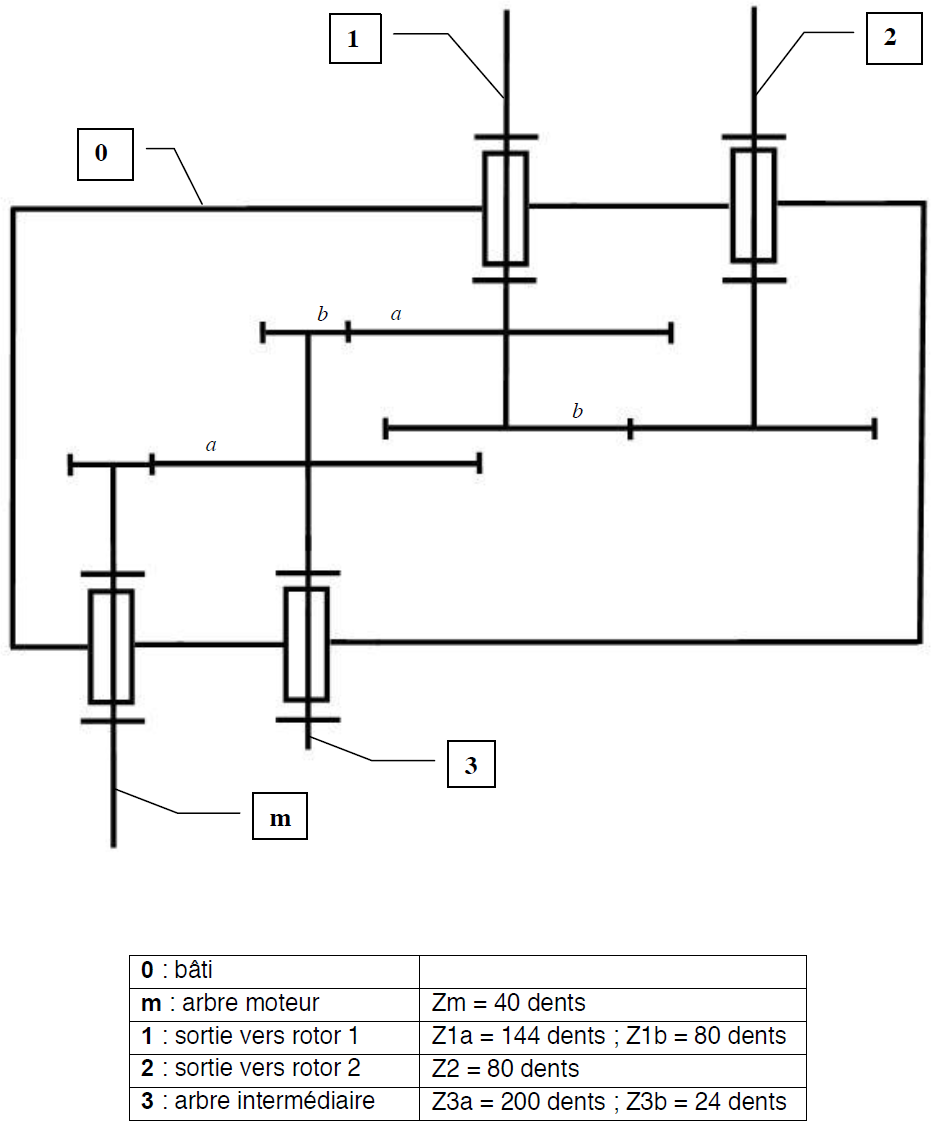
\includegraphics[width=.6\textwidth]{images/reducteur}
\end{center}
}


% Question II.A.3
\subparagraph{}
\textit{Donner la valeur algébrique des rapports de réduction $r_1=\dfrac{\omega_1}{\omega_m}$ et $r_2=\dfrac{\omega_2}{\omega_m}$ en fonction des nombres de dents $Z_i$. Faire les applications numériques.}
\ifthenelse{\boolean{prof}}{
\begin{corrige}
$r_1=\dfrac{\omega_2}{\omega_m} = (-1)^n \dfrac{Z_m\cdot Z_{3b}\cdot Z_{1b}}{ Z_{3a}\cdot Z_{1a}\cdot Z_2} = -\dfrac{40\cdot 24 \cdot 80}{200 \cdot 144 \cdot 80} =-0,033 $ 

$r_2=\dfrac{\omega_1}{\omega_m} = (-1)^n \dfrac{Z_m\cdot Z_{3b}}{ Z_{3a}\cdot Z_{1a}}
= 0,033$ 
\end{corrige}}{}

% Question II.A.4
\subparagraph{}
\textit{Quelle doit être la fonction de transfert $K_a$ de l'adaptateur de consigne (case $a$) si l'on veut que l’écart $\varepsilon$ soit nul quand la vitesse $\omega_1$ est égale à la vitesse de consigne $\omega_c$ ? Remplir la case $a$ du schéma bloc précédent.}
\ifthenelse{\boolean{prof}}{
\begin{corrige}
On a : $\varepsilon(p)= a \cdot \Omega_c(p) -k_g \Omega_m(p) = a \cdot \Omega_c(p) -k_g \dfrac{\Omega_1(p)}{r_1}=0$. Or dans les conditions indiquées ci-dessus, on souhaite que $\varepsilon(p)=0$ lorsque $\Omega_m(p) = \Omega_1(p)$; donc : 
$a \cdot \Omega_c(p) -k_g \dfrac{\Omega_c(p)}{r_1}=0 \Longleftrightarrow a -k_g \dfrac{1}{r_1}=0 \Longleftrightarrow a = \dfrac{k_g}{r_1}$
\end{corrige}}{}

Dans un premier temps nous considèrerons que le correcteur est proportionnel de fonction de transfert $k_c$.


% Question II.A.5
\subparagraph{}
\textit{
\begin{itemize}
\item Déterminer l'expression littérale de la fonction de transfert $H(p)=\dfrac{\Omega_1(p)}{\Omega_c(p)}$ de suivi de consigne ($C_r(p) = 0$) en fonction de $A$, $R$, $L$, $J$, $k_i$, $k_e$, $k_g$ et $k_c$.
\item La mettre sous la forme $H(p)=\dfrac{K}{1+\dfrac{2\xi}{\omega_0}p+\dfrac{1}{\omega_0^2}p^2}$ et identifier les constantes $K$, $\xi$ et $\omega_0$.
\end{itemize}}
\ifthenelse{\boolean{prof}}{
\begin{corrige}
D'une part, on a :
$$
\dfrac{\Omega_m(p)}{U(p)} = \dfrac{\dfrac{1}{R+Lp}\cdot k_i\cdot\dfrac{1}{Jp}}{1+\dfrac{1}{R+Lp}\cdot k_i\cdot\dfrac{1}{Jp} k_e}
=\dfrac{k_i}{(R+Lp)Jp+ k_ik_e}
$$

D'autre part :

$$H(p)=\dfrac{\Omega_1(p)}{\Omega_c(p)}
=\dfrac{k_g}{r_1} \cdot \dfrac{k_c A \dfrac{k_i}{(R+Lp)Jp+ k_ik_e} }{1+k_c A k_g \dfrac{k_i}{(R+Lp)Jp+ k_ik_e}}\cdot r_1
= \dfrac{k_g k_c A k_i}{RJp+LJp^2+ k_ik_e+k_c A k_g k_i}
$$
$$H(p)=\dfrac{\dfrac{k_g k_c A }{k_e+k_c Ak_g }}{\dfrac{RJ}{k_ik_e+k_c Ak_g k_i}p+\dfrac{LJ}{k_ik_e+k_c Ak_g k_i}p^2+ 1}
$$
Par identification :
$$
\left\{
\begin{array}{l}
K = \dfrac{k_g k_c A }{k_e+k_c Ak_g } \\
\dfrac{1}{\omega_0^2} = \dfrac{LJ}{k_ik_e+k_c Ak_g k_i} \\
\dfrac{2\xi}{\omega_0} = \dfrac{RJ}{k_ik_e+k_c Ak_g k_i}
\end{array}
\right.
\Longleftrightarrow
\left\{
\begin{array}{l}
K = \dfrac{k_g k_c A }{k_e+k_c Ak_g } \\
\omega_0 = \sqrt{\dfrac{k_ik_e+k_c Ak_g k_i}{LJ}} \\
\xi= \dfrac{1}{2}\dfrac{R\sqrt{J}}{\sqrt{L}\sqrt{k_ik_e+k_c Ak_g k_i}}
\end{array}
\right.
$$
\end{corrige}}{}


\subsection{Étude de l'asservissement de vitesse}

\ifthenelse{\boolean{prof}}{}{
\begin{obj}
Choisir et régler un correcteur pour répondre au cahier des charges.
\end{obj}

Pour cette partie, on utilisera le schéma-bloc à retour unitaire suivant :

\begin{center}
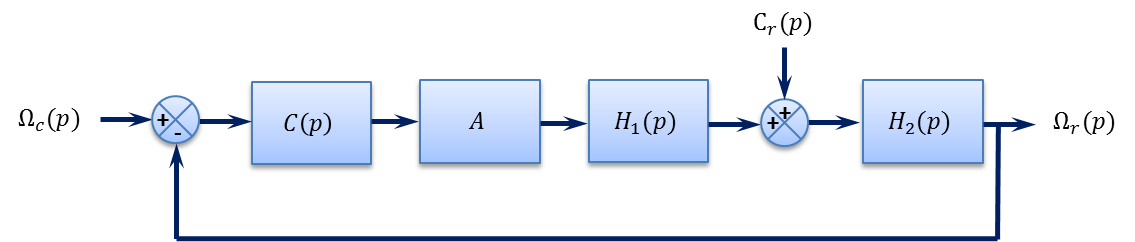
\includegraphics[width=.8\textwidth]{images/SchemaBloc2}
\end{center}


Avec  $H_1(p)=\dfrac{3000}{1+1,6\cdot10^{-2}p}$, $H_2(p)=\dfrac{5,7\cdot 10^{-5}\left(1+1,6\cdot10^{-2}p \right)}{1+2,9\cdot 10^{-2}p+ 4,6\cdot 10^{-4} p^2}$  et $A = 5$ (sans unité). Les valeurs numériques sont dans les unités du système international.
 
\begin{center}
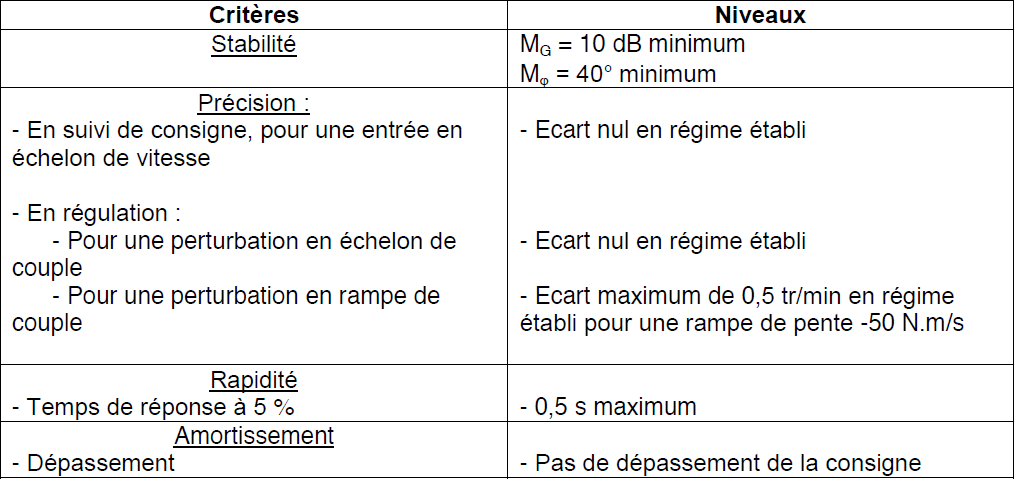
\includegraphics[width=.6\textwidth]{images/Criteres}
\end{center}
%Le cahier des charges impose les conditions suivantes :
%Critères	Niveaux
%Stabilité	MG = 10 dB minimum
%M = 40° minimum
%Précision :
%- En suivi de consigne, pour une entrée en échelon de vitesse
%
%- En régulation :
%      - Pour une perturbation en échelon de couple
%      - Pour une perturbation en rampe de couple
%	
%- Ecart nul en régime établi
%
%
%
%- Ecart nul en régime établi
%
%- Ecart maximum de 0,5 tr/min en régime établi pour une rampe de pente -50 N.m/s
%Rapidité
%- Temps de réponse à 5 %	
%- 0,5 s maximum
%Amortissement
%- Dépassement	
%- Pas de dépassement de la consigne

\begin{rem}
\begin{itemize}
\item La perturbation en échelon de couple modélise une variation brusque du couple résistant au niveau des rotors due à la mise en action du fouloir.
\item La perturbation en rampe de couple modélise une variation lente du couple résistant liée à la variation de température du mélange.
\end{itemize}
\end{rem}

Le diagramme de Bode de la fonction de transfert en boucle ouverte du système non corrigé ($C(p) = 1$) est donné ci-dessous.
 
\begin{center}
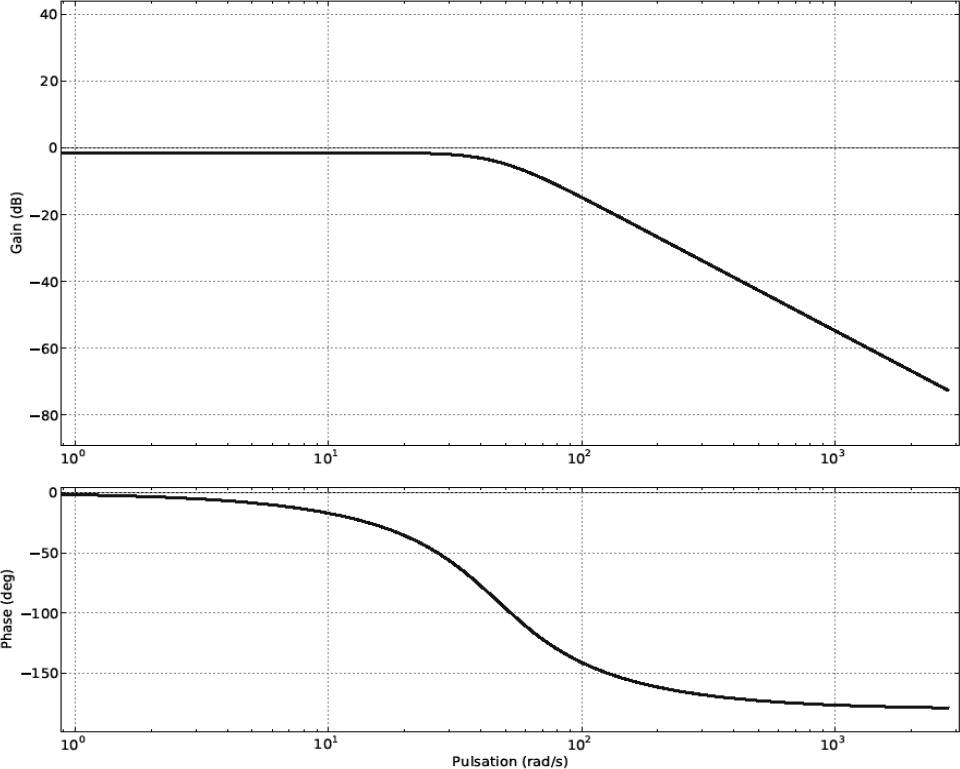
\includegraphics[width=.8\textwidth]{images/Bode}
\end{center}
}
%% Question II.D.1
%\subparagraph{}
%\textit{Le système modélisé ainsi est-il stable ? Justifier votre réponse.}

% Question II.D.2
\subparagraph{}
\textit{Si l'on considère dans un premier temps que le correcteur est proportionnel de fonction de transfert $C(p) = K$, donner la valeur que prend l'écart (en fonction de $a$, $b$, $c$ et $K$ s’il est constant) dans chacun des trois cas proposés. 
%(on ne demande pas de développer de calculs sur la copie). 
Le cahier des charges est-il respecté ?}
\ifthenelse{\boolean{prof}}{
\begin{corrige}
%D'une part, considérons que $C_r(p)=0$ :
%$$
%\dfrac{\Omega_r(p)}{\Omega_c(p)} 
%= \dfrac{AC(p)H_1(p)H_2(p)}{1+AC(p)H_1(p)H_2(p)}
%$$
%D'une part, considérons que $\Omega_c(p)=0$ :
%$$
%\dfrac{\Omega_r(p)}{C_r} 
%= \dfrac{H_2(p)}{1+AC(p)H_1(p)H_2(p)}
%$$
Calculons la fonction écart : 
$$
\varepsilon(p)
= \Omega_c(p)-\Omega_r(p) 
= \Omega_c(p) - \left( C_r(p)+\varepsilon(p)AC(p)H_1(p)\right)H_2(p) 
= \Omega_c(p)- C_r(p)H_2(p)-\varepsilon(p)AC(p)H_1(p)H_2(p) 
$$
On a alors :
$$
\varepsilon(p) = \dfrac{\Omega_c(p)-C_r(p)H_2(p)}{1+AC(p)H_1(p)H_2(p)}
$$

Dans le premier cas, $\Omega_c(p)=\dfrac{a}{p}$ et $C_r(p)=0$; donc :
$$
\varepsilon_s = \underset{p\to0} {\lim}p \cdot \dfrac{a}{p} \dfrac{1}{1+AKH_1(p)H_2(p)} = \dfrac{a}{1+3000\cdot 5 \cdot K\cdot 5,7\cdot 10^{-5}}
= \dfrac{a}{1+0,855\cdot K}
$$

Dans le second cas, $\Omega_c(p)=0$ et $C_r(p)=\dfrac{b}{p}$; donc :
$$
\varepsilon_s = \underset{p\to0} {\lim}p \cdot \dfrac{-b}{p} \dfrac{H_2(p)}{1+AC(p)H_1(p)H_2(p)} 
=-b\dfrac{5,7\cdot 10^{-5}}{1+0,855\cdot K}
$$

Dans le troisième cas, $\Omega_c(p)=0$ et $C_r(p)=\dfrac{c}{p^2}$; donc :
$$
\varepsilon_s =\underset{p\to0} {\lim}p \cdot \dfrac{-c}{p^2} \dfrac{H_2(p)}{1+AC(p)H_1(p)H_2(p)} = -\infty
$$
\end{corrige}}{}

\ifthenelse{\boolean{prof}}{}{
\begin{center}
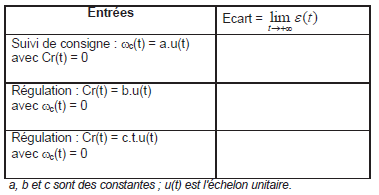
\includegraphics[width=.4\textwidth]{images/qiid2}
\end{center}}
\subparagraph{}
\textit{Dans quel(s) cas le cahier des charges est il-respecté sur le critères de précision ?}
\ifthenelse{\boolean{prof}}{
\begin{corrige}
Le cahier des charges n'est pas respecté. 
\end{corrige}}{}


% Question II.D.3
\subparagraph{}
\textit{Parmi les quatre correcteurs proposés,
 %cocher celui (ou ceux) qui peut (peuvent) 
quels sont ceux qui permettent de répondre aux trois critères de précision du cahier des charges.}
\ifthenelse{\boolean{prof}}{
\begin{corrige}
Afin d'avoir un écart statique nul dans pour les 3 critères, il est nécessaire qu'il y ait un intégrateur en amont de la perturbation. Il faudra donc avoir recours aux correcteurs 2 ou 4. 
\end{corrige}}{}
\ifthenelse{\boolean{prof}}{}{
\begin{center}
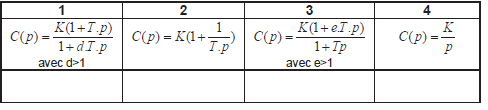
\includegraphics[width=.6\textwidth]{images/qiid3}
\end{center}}

Pour la suite nous utiliserons un correcteur de fonction de transfert  $C(p)=K\dfrac{1+Tp}{Tp}$

\begin{rem}
Ce correcteur est appelé proportionnel intégral.
\end{rem}

% Question II.D.4
\subparagraph{}
\textit{Tracer le diagramme de Bode (asymptotique et allure du diagramme réel) du correcteur seul. Indiquer les pentes et points caractéristiques en fonction de $K$ et $T$.}
\ifthenelse{\boolean{prof}}{
\begin{corrige}
\begin{center}
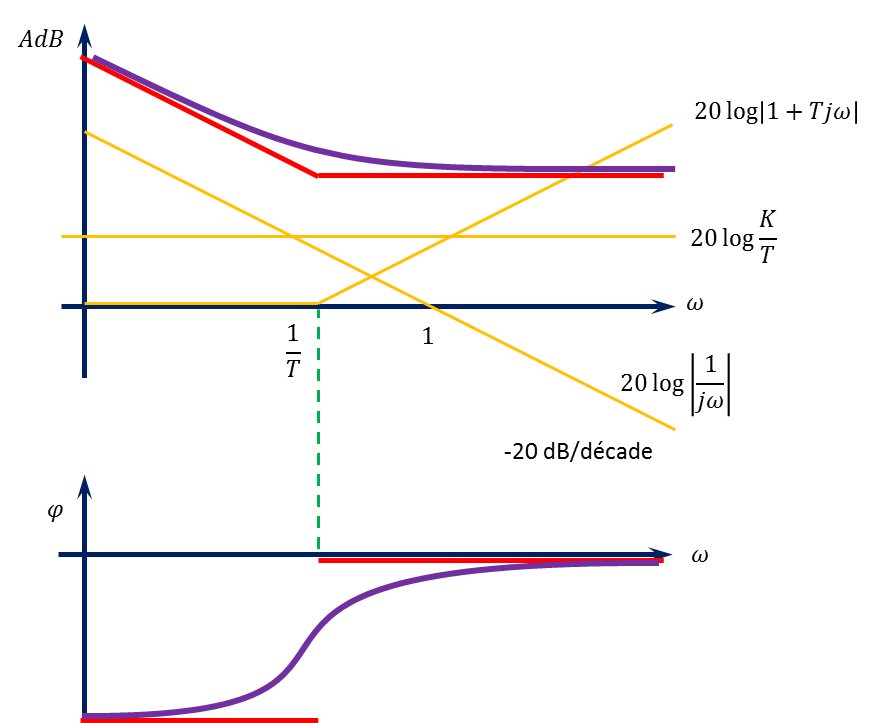
\includegraphics[width=.6\textwidth]{images/corrige_bode_correcteur}
\end{center}
\end{corrige}}{}

On choisit la valeur de $T$ de telle façon que la valeur de la pulsation conduisant à un déphasage de $-45\textdegree$ pour le correcteur seul soit dix fois plus petite que la pulsation pour laquelle la FTBO non corrigée présente un déphasage de $-90\textdegree$.

% Question II.D.5
\subparagraph{}
\textit{
\begin{itemize}
\item Déterminer la valeur de $T$ correspondante.
\item Tracer le diagramme asymptotique de Bode de la FTBO corrigée avec $K = 1$ et votre valeur de $T$. Indiquer les pentes et points caractéristiques.
\end{itemize}}
\ifthenelse{\boolean{prof}}{
\begin{corrige}
D'après le tracé de la FTBO, la phase est de -90\textdegree lorsque $\omega=45\; rad/s$. On doit donc choisir $T$ tel que $1/T=4,5\; rad/s$. On a donc $T=0,22\; s$.  

\end{corrige}}{}
\ifthenelse{\boolean{prof}}{}{
\begin{center}
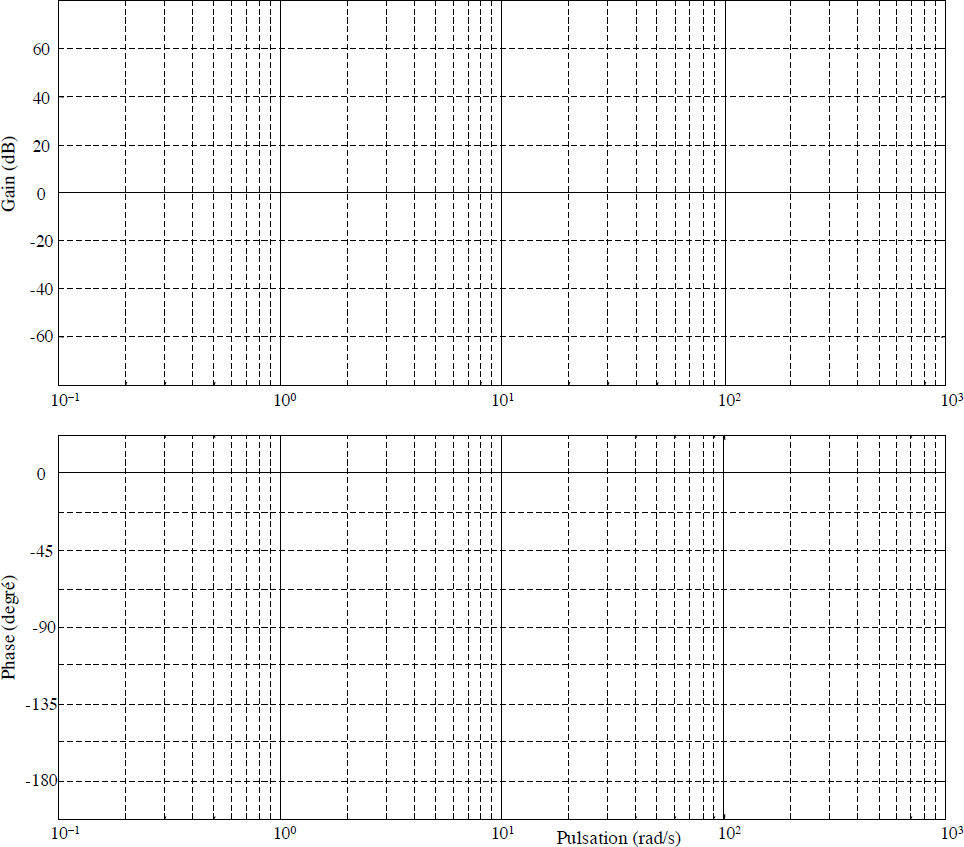
\includegraphics[width=.8\textwidth]{images/qiid5}
\end{center}

%On donne, sur le cahier réponses, le diagramme de Black de la FTBO corrigée avec $T$ déterminé à la question précédente et $K = 1$.

% Question II.D.6
%\subparagraph{}
%\textit{Déterminer la plus grande valeur de $K$ (notée $K_{stab}$) permettant de satisfaire au critère de stabilité. Vous porterez sur la courbe les tracés que vous jugerez utiles.}

\begin{rem}
On montre qu'au maximum, $K_{stab}=4,5$.
\end{rem}

On donne ci-dessous les courbes de la réponse du système à une entrée en échelon unitaire ($\omega_c(t) = u(t)$) pour $K$ prenant les valeurs  $\{1; 2 ; 3 ; 3,5 ; 4\}$.
}
% Question II.D.7 :
\subparagraph{}
\textit{
\begin{itemize}
\item La valeur de $K_{stab}$ est-elle compatible avec les critères de précision en suivi de consigne, d'amortissement et de rapidité ? Justifiez votre réponse.
\item Choisir pour $K$ une valeur permettant de respecter à la fois les critères de stabilité, amortissement, rapidité et précision en suivi de consigne. Vous justifierez vos réponses et porterez sur la courbe les tracés que vous jugerez utiles.
\end{itemize}}
\ifthenelse{\boolean{prof}}{
\begin{corrige}
\begin{minipage}[c]{.47\linewidth}
Le cahier des charges indique que pour une sollicitation à un échelon l'écart statique doit être nul en régime permanent, que le temps de réponse à 5\% doit être inférieur à 0,5 s et que la consigne ne doit pas être dépassée. 

D'après le réseau de courbe proposé, il semble que $K$ doivent être inférieur à 3 pour ne pas dépasser la consigne. Par ailleurs, le cas $K=3$ a un temps de réponse à 5\% et semble présenter un écart statique nul. 
\end{minipage}\hfill
\begin{minipage}[c]{.47\linewidth}
\begin{center}
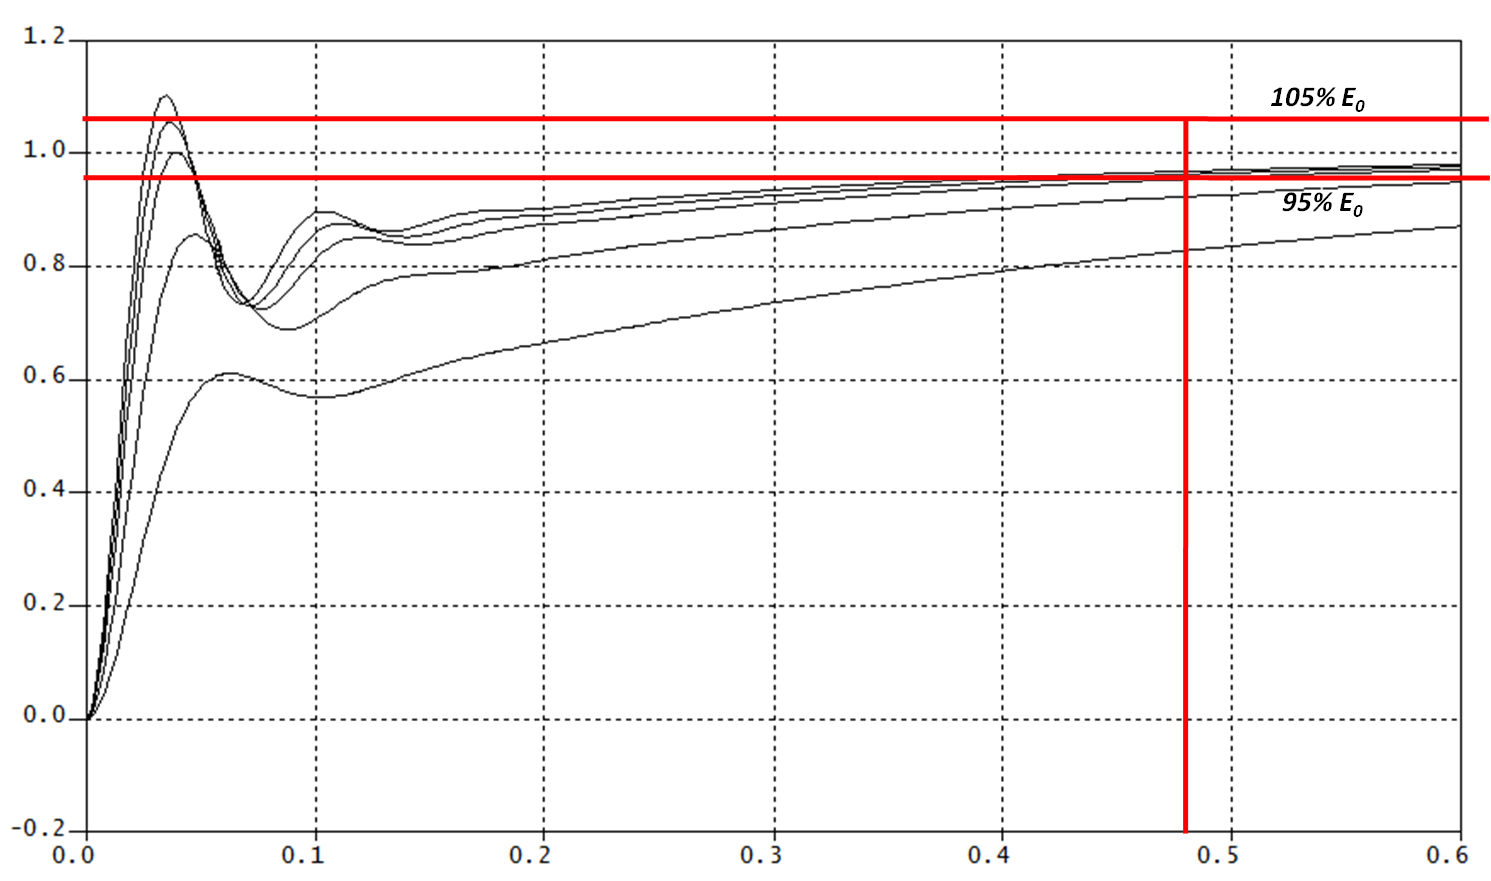
\includegraphics[width=.95\textwidth]{images/corrige_K}
\end{center}
\end{minipage}

\end{corrige}}{}
\ifthenelse{\boolean{prof}}{}{
\begin{center}
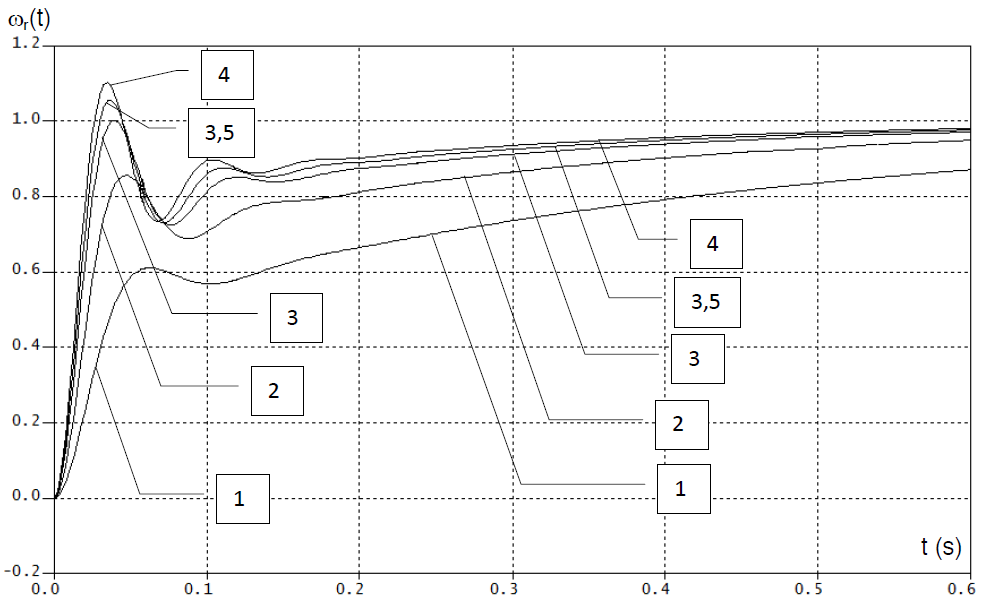
\includegraphics[width=.8\textwidth]{images/qiid7}
\end{center}


Le correcteur ayant été dimensionné, le schéma-bloc peut se mettre sous la forme suivante :
Avec $F(p)=\dfrac{2,25\cdot 10^5 \left(1+0,2p\right)}{p\left(1+1,6\cdot 10^{-2}p\right)}$ et $H_2(p)=\dfrac{5,7\cdot 10^{-5}\left(1+1,6\cdot 10^{-2}p\right) }{1+2,9\cdot 10^{-2}p+4,6\cdot 10^{-4}p^2}$. Les valeurs numériques sont dans les unités du système international.

Nous nous intéressons maintenant à la précision en régulation du système modélisé ainsi. L'étude sera donc faite pour une consigne nulle $\omega_c(t) = 0$.
}

% Question II.D.8
\subparagraph{}
\textit{Déterminer l'expression de $\varepsilon(p)$ en fonction de $C_r(p)$, $F(p)$ et $H_2(p)$.}
\ifthenelse{\boolean{prof}}{
\begin{corrige}
On a vu que $
\varepsilon(p) = \dfrac{\Omega_c(p)-C_r(p)H_2(p)}{1+AC(p)H_1(p)H_2(p)}$. Si $\Omega_c(p) = 0$ :
$$
\varepsilon(p) = \dfrac{-C_r(p)H_2(p)}{1+AC(p)H_1(p)H_2(p)}
$$

\end{corrige}}{}

% Question II.D.9
\subparagraph{}
\textit{Que vaut $\varepsilon_1 = \underset{t\to +\infty}{\lim} \varepsilon(t)$ pour une perturbation en échelon $C_r(t) = b u(t)$ ? Justifier votre réponse et conclure quant au respect du cahier des charges.}
\ifthenelse{\boolean{prof}}{
\begin{corrige}
$$
\varepsilon_1 
= \underset{t\to +\infty}{\lim} \varepsilon(t)
= \underset{p\to 0}{\lim} p\dfrac{-C_r(p)H_2(p)}{1+AC(p)H_1(p)H_2(p)}
= \underset{p\to 0}{\lim} \dfrac{-bH_2(p)}{1+AC(p)H_1(p)H_2(p)}
= 0
$$
\end{corrige}}{}

% Question II.D.10
\subparagraph{}
\textit{Déterminer $\varepsilon_2 = \underset{t\to +\infty}{\lim} \varepsilon(t)$ pour une perturbation en rampe $C_r(t) = c t u(t)$. Le cahier des charges est-il respecté (justifier par l'application numérique sur $\varepsilon_2$) ?}
\ifthenelse{\boolean{prof}}{
\begin{corrige}
$$
\varepsilon_2
= \underset{p\to 0}{\lim} \dfrac{-(c/p)H_2(p)}{1+AC(p)H_1(p)H_2(p)} = -\dfrac{c}{2,25\cdot 10^5}
$$
Pour $c=50$, $\varepsilon_2 =  2,2 \cdot 10^{-4} rad/s=0,0021 tr/min$. Le cahier des charges est respecté. 
\end{corrige}}{}


\section{Étude de la chaîne fonctionnelle d'actionnement du fouloir}
\ifthenelse{\boolean{prof}}{}{
\begin{obj}
Analyser la commande logique de la chaîne d’énergie pneumatique d’ouverture et de fermeture de la chambre de mélangeage participant aux exigences 1.1, 1.2 et 1.4. Vérifier les performances dynamiques de cette chaîne d’énergie. Analyser la structure mécanique de la solution hydraulique alternative.
\end{obj}
}
\subsection{Étude de la commande}
\ifthenelse{\boolean{prof}}{}{
\begin{obj}
Déterminer les équations de commande du vérin actionnant le fouloir.
\end{obj}

Le fouloir actionné par un vérin double-effet monte et descend sous les actions de pression pneumatique et de pesanteur. Pour certains cycles de production de mélange de caoutchouc il est possible de commander le fouloir en utilisant une pression pneumatique haute (6,5 bars) ou basse (3,7 bars). On donne en annexe A le schéma pneumatique de l’installation permettant la mise en mouvement du fouloir.
}

%Question III.A.1
\subparagraph{}
\textit{A partir des informations figurant sur le schéma pneumatique, exprimer les équations logiques définissant respectivement, la commande de la descente en haute pression $D_h$, la commande de la descente en basse pression $D_b$ et la commande de montée en haute pression $M_h$. Ces expressions seront données en fonction des variables logiques $V1$, $V2$, $V3$ et $V4$ de commande électrique des distributeurs.}
\ifthenelse{\boolean{prof}}{
\begin{corrige}
On a :
$$D_h=V_1 \cdot \overline{V_2}\cdot V_3 \cdot  \overline{V_4}
\quad
D_b=V_1 \cdot \overline{V_2}\cdot \overline{V_3} \cdot  \overline{V_4}
\quad
M_h=\overline{V_1} \cdot V_2 \cdot V_3 \cdot  \overline{V_4}$$



\end{corrige}}{}

%Question III.A.2
\subparagraph{}
\textit{Proposer une commande A permettant d’immobiliser le fouloir dans une position quelconque (à la compressibilité de l’air près). Cette commande pourra être exprimée en fonction des variables logiques  $V1$, $V2$, $V3$ et $V4$.}
\ifthenelse{\boolean{prof}}{
\begin{corrige}
$$A=\overline{V_1} \cdot \overline{V_2} \cdot \overline{V_3} \cdot  V_4$$
\end{corrige}}{}


\subsection{Étude du mouvement du fouloir}
\ifthenelse{\boolean{prof}}{}{
\begin{obj}
Vérifier que la dynamique du fouloir répond au cahier des charges (Voir annexe A pour le paramétrage et les caractéristiques dimensionnelles).
\end{obj}

\begin{rem}
Le cahier des charges impose les conditions suivantes :
\begin{itemize}
\item temps d'ouverture de la chambre : 1 seconde maximum;
\item variation de hauteur du fouloir en cours de mélangeage : 30 cm maximum.
\end{itemize}

\end{rem}

%
%On veut, dans un premier temps, évaluer la durée de la phase de montée du fouloir.
%Partant de la position basse on utilise la commande $Mh$ de montée. La pression d’air est donc $Pi = 6,5\;bars$ dans la chambre inférieure alors que la pression de fuite dans la chambre supérieure est $Ps = 0,5 \;bars$.

On considère :
\begin{itemize}
\item un coefficient de frottement visqueux de l’ensemble piston-tige-fouloir/guidage : $f = 5000 N/(m/s)$;
\item une course utile du vérin de la position basse à la position haute :  $l_0= 1\;m$;
\item $k = 85000 \; N/m$.
\end{itemize}
}
\subsection{Étude du mouvement du fouloir}
\ifthenelse{\boolean{prof}}{}{
On note $F(p)$ la transformée de Laplace de $F(t) - F_0$.

\begin{rem}
En appliquant  le théorème de la résultante dynamique en projection sur $\vect{z_0}$ à l'ensemble \{fouloir+piston+tige\}, on montre que :
$$
a\ddot{z}+b\dot{z}+cz = F(t)-F(0)
$$

avec $a=M$, $b=f$, $c=k$.
\end{rem}}
% Question III.B.8
\subparagraph{}
\textit{En considérant que toutes les conditions initiales sont nulles, déterminer l'expression littérale de la fonction de transfert $Z(p)/F(p)$. Faire l’application numérique.}
\ifthenelse{\boolean{prof}}{
\begin{corrige}
On a :
$$
\dfrac{Z(p)}{F(p)} = \dfrac{1}{Mp^2+fp+k}=\dfrac{\dfrac{1}{k}}{\dfrac{M}{k}p^2+\dfrac{f}{k}p+1}
$$

Avec : 
$$
\left\{
\begin{array}{l}
K= \dfrac{1}{k} = 1,17\cdot 10^{-5} m/N \\
\omega_0 = \sqrt{\dfrac{k}{M}} = 4,9 rad/s\\
\xi = \dfrac{f\omega_0}{2k}= 0,14
\end{array}
\right.
$$
\end{corrige}}{}

% Question III.B.9
\subparagraph{}
\textit{\begin{itemize}
\item En utilisant l’abaque fourni en annexe B, tracer l’allure de la courbe $z(t)$ de position du fouloir soumis à l’excitation en échelon d’effort de $10\,000\; N$.
\item Mettre en place sur celle-ci les valeurs numériques caractéristiques.
\item Conclure quant au respect du cahier des charges.
\end{itemize}}
\ifthenelse{\boolean{prof}}{
\begin{corrige}
Pour un échelon de 10 000 N, la valeur finale tend vers 0,11 m, le premier dépassement est de près de 70\% soit approximativement 0,2 m.
\begin{center}
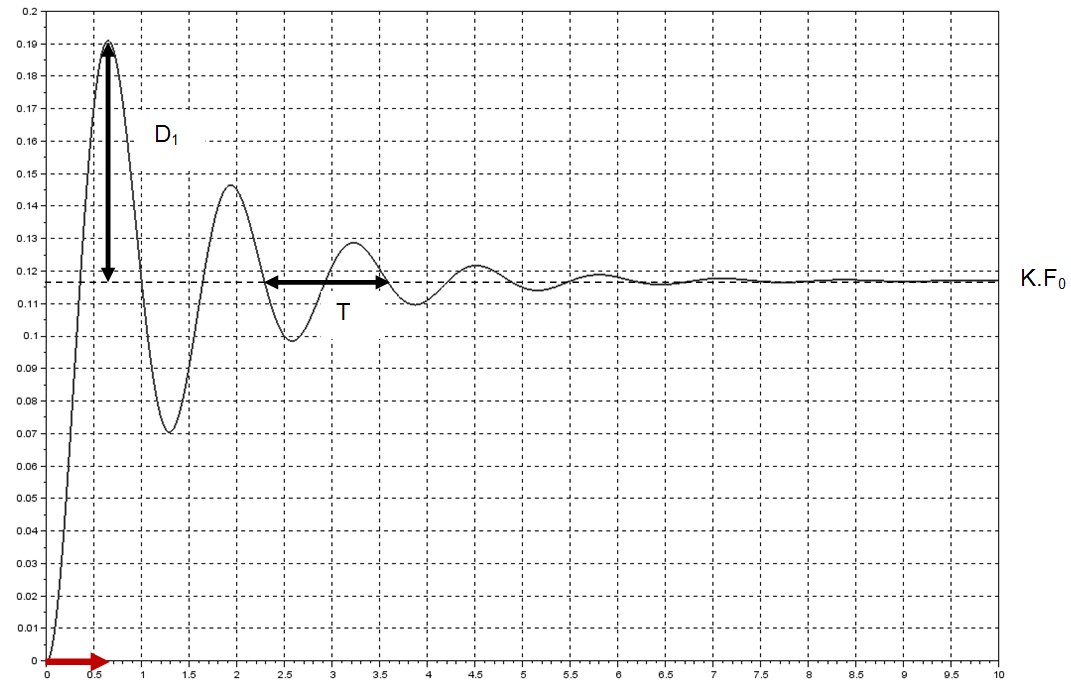
\includegraphics[width=.8\textwidth]{images/corrige_mvt}
\end{center}
\end{corrige}}{}

%
%Ce mouvement d’oscillation permet d’éviter une surpression au sein du mélange et ainsi un échauffement excessif. Toutefois, il ne permet pas un contrôle précis de la pression et de la position du fouloir nécessaires pour certains types de mélanges. Ces mélanges imposent une variation de hauteur du fouloir en position basse de l’ordre du centimètre. La solution à ce nouveau cahier des charges est le passage à une technologie hydraulique.
%
%Le fouloir est alors actionné par deux vérins hydrauliques (formés des pièces 6, 6’, 7 et 7’) comme illustré sur l’annexe F. Les efforts à développer étant très importants, la structure mécanique doit être suffisamment rigide.
%
\ifthenelse{\boolean{prof}}{}{
\section*{Annexe A}
\begin{center}
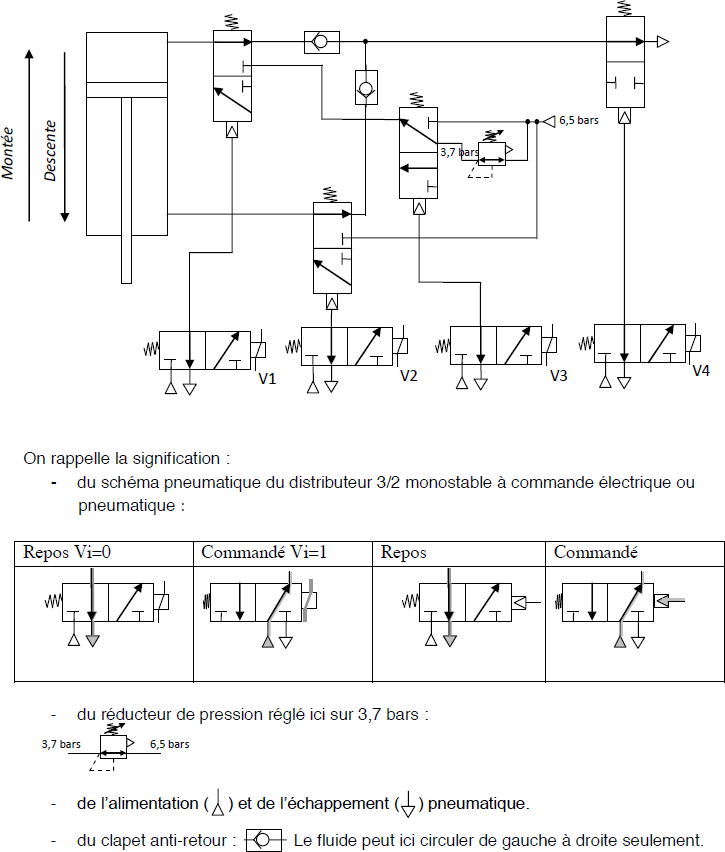
\includegraphics[width=.8\textwidth]{images/annexeB_1}

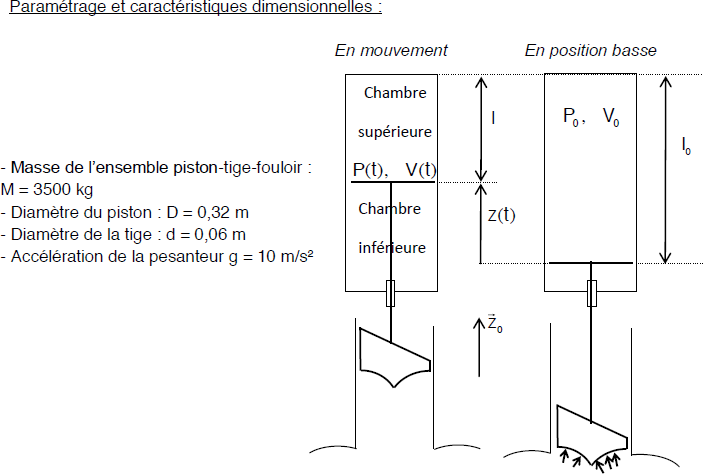
\includegraphics[width=.8\textwidth]{images/annexeB_2}
\end{center}

\section*{Annexe B}
\begin{center}
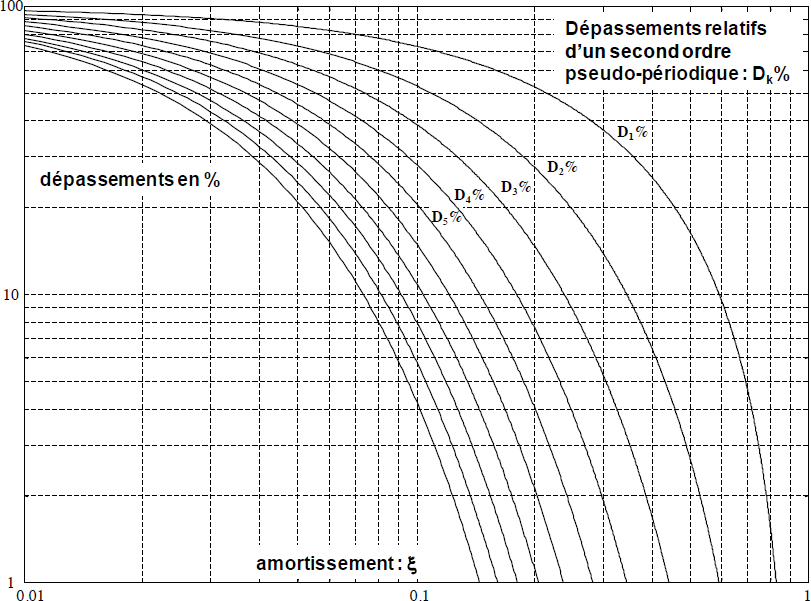
\includegraphics[width=.8\textwidth]{images/annexeE}
\end{center}
}
\end{document}


